\documentclass[12pt,a4paper]{article}
\usepackage[utf8]{inputenc}
\usepackage[T1]{fontenc}
\usepackage{comment}
\date{} 
\usepackage[spanish]{babel}
\usepackage{amsmath}
\usepackage{amsfonts}
\usepackage{rotating} %table rotate
\usepackage{array}
\usepackage{lscape} %pagina horizontal


\usepackage{booktabs, multirow} % for borders and merged ranges
\usepackage{soul}% for underlines
\usepackage[table,hyperref]{xcolor} % for cell colors  %color rgb para links
\usepackage{changepage,threeparttable} % for wide tables
\usepackage{longtable}

\usepackage{tcolorbox} %cajas de definiciones
\usepackage{color}%resaltador
\usepackage{soul}%resaltador
\usepackage{booktabs, multirow}%tabla ultimo agregado

\usepackage{enumitem}%separacion de las listas
\setlist[itemize]{noitemsep, topsep=1pt}%separacion de las listas
\setlist[enumerate]{noitemsep, topsep=1pt}%separacion de las listas


%bibliografía
\usepackage[maxbibnames=99, sorting=none, backend=bibtex]{biblatex}
\addbibresource{bibliogr.bib}
%\usepackage[nottoc]{biblatex}

%para crear sub sub sub titulos
\makeatletter
\renewcommand\paragraph{\@startsection{paragraph}{4}{\z@}%
            {-2.5ex\@plus -1ex \@minus -.25ex}%
            {1.25ex \@plus .25ex}%
            {\normalfont\normalsize\bfseries}}
\makeatother
\setcounter{secnumdepth}{4} % how many sectioning levels to assign numbers to
\setcounter{tocdepth}{4}    % how many sectioning levels to show in ToC

\usepackage[none]{hyphenat} %para que no corte las palabras al final del renglon
\usepackage{amssymb}
\usepackage{graphicx}
\usepackage{subfigure}

%reiniciar los contadores de figuras
\usepackage{chngcntr}
\counterwithin{figure}{section}
\counterwithin{table}{section}

\usepackage{appendix}
\renewcommand{\appendixpagename}{Anexos}


\usepackage{fancyhdr}%encabezado y pie de pagina
\usepackage{caption}
\usepackage{mwe}
\usepackage{url} %url
\usepackage{hyperref} %indice con hipervínculo
\hypersetup{
    colorlinks=true,
    linkcolor=[RGB]{4,41,64},
    filecolor=white,      
    urlcolor=blue,
    citecolor=blue,
}
\usepackage{float} 
\usepackage{mathpazo} % Palatino font
\usepackage[left=2.50cm, right=2.50cm, top=2.50cm, bottom=2.50cm]{geometry}
\author{Caamiña, Daniela \and Yapura, Cristian}
\title{Trabajo final \\Automatización industrial}
\graphicspath{ {images/} }


%encabezado y pie de pagina
\pagestyle{fancy}
\fancyhead[L]{}
\fancyhead[R]{}
\fancyhead[C]{\textbf{Automatización Industrial - Trabajo Final}}
\fancyfoot[L]{}
\fancyfoot[C]{\thepage}
\fancyfoot[R]{Autores: Caamiña - Yapura}
\renewcommand{\headrulewidth}{0.4pt}
\renewcommand{\footrulewidth}{2pt}

	
\begin{document}
\begin{titlepage} %Carátula 			
	\newcommand{\HRule}{\rule{\linewidth}{0.5mm}}
	\center % Centre everything on the page		
	\textsc{\LARGE Universidad Nacional de la Patagonia San Juan Bosco}\\[1.5cm]
	\textsc{\Large Automatización Industrial}\\[0.5cm]
	\textsc{\large Trabajo Final}\\[0.5cm]
	\HRule\\[0.4cm]
	\huge\bfseries{Banco de pruebas para control de presión o caudal}\\[0.2cm]
	\HRule\\[1.5cm]
	\begin{minipage}{0.4\textwidth}
		\begin{flushleft}
			\large
			\textit{Alumnos}\\
			\textsc{Caamiña,} Daniela \\
			\textsc{Yapura,} Cristian
		\end{flushleft}
	\end{minipage}
	\begin{minipage}{0.4\textwidth}
		\begin{flushright}
			\large
			\textit{Docentes}\\
			Ing. \textsc{Lorenc,} Marcelo \\
			Dr. \textsc{Peña,} Ramiro
		\end{flushright}
	\end{minipage}
	\vfill\vfill\vfill
	\large{MES AÑO}
	\vfill\vfill
	
\includegraphics[width=0.2\textwidth]{unpsjb.png}\\[1cm]
	\vfill
\end{titlepage}

\newpage
	


\section*{Agradecimientos}
\vspace{6cm}

	\begin{flushleft}
		\textit{	Agradecemos a los docentes de la cátedra de Automatización Industrial que nos dieron la posibilidad de realizar este proyecto y nos facilitaron los dispositivos necesarios para la implementación. A Gerardo Arthz quien diseñó y fabricó el soporte para el motor y variador de velocidad. También al equipo del taller de soldadura y tornería dependientes del departamento de Ingeniería Mecánica quienes fabricaron el soporte de la bomba y ayudaron con el acople del motor- bomba.}\\
	\vspace{3cm}
	\textit{	Al ser la última materia para recibirnos de Ingenieros Electrónicos, y tal como dijimos en el proyecto final de carrera, este trabajo está especialmente dedicado a nuestros padres quienes nos brindaron el apoyo y estuvieron en cada paso de nuestra carrera universitaria, también agradecemos infinitamente a nuestros hermanos, novia/o, familia y amigos quienes fueron nuestro soporte y que nos acompañaron durante todos los años de estudio. Reconocemos y agradecemos a cada persona que de alguna forma nos ayudó a transitar este camino.}
	\end{flushleft}



\newpage

\tableofcontents
\newpage

\listoffigures
\newpage

\listoftables
\newpage
\section*{Lista de Acrónimos}
\noindent %desactiva sangria solo para este parrafo
\textbf{CS :} \textit{Controlador de velocidad}\\
\textbf{DTM :} \textit{Gestor de tipos de dispositivo}\\
\textbf{FT :} \textit{Transmisor de caudal}\\
\textbf{FV :} \textit{Válvula reguladora de caudal}\\
\textbf{HMI :} \textit{Interfaz hombre-máquina}\\
\textbf{ISA :} \textit{Sociedad de Instrumentos de América (EEUU)}\\
\textbf{MFE :} \textit{Bloques de fundiones de movimiento}\\
\textbf{OFS :} \textit{OPC Factory Server, software de Schneider}\\
\textbf{P \& ID :} \textit{Diagrama de cañerías e instrumentación}\\
\textbf{PIT :} \textit{Transmisor con indicador de presión}\\
\textbf{PLC :} \textit{Controlador Lógico Programable}\\
\textbf{RTD :} \textit{Detectores de temperatura resistivos}\\
\textbf{SCADA :} \textit{Supervisión, Control y Adquisición de Datos}\\ %desactiva sangria solo para este parrafo
\textbf{SDO :} \textit{Objetos o mensajes de servicio}\\
\textbf{TE :} \textit{Elemento primario de temperatura}\\
\textbf{UNPSJB:} \textit{Universidad Nacional de la Patagonia San Juan Bosco}\\
\textbf{VSD :} \textit{Variador de velocidad}\\

\newpage


\sloppy %para justificar los párrafos

\section{Introducción}
En el Laboratorio de Fluidos de la Universidad, se utiliza el Túnel de Viento para realizar el contraste de anemómetros y experimentos para distintas materias. Gran parte de estas aplicaciones requieren que se conozca la velocidad del fluido (aire). Por lo tanto, variación de presión, humedad, presión atmosférica y temperatura son variables requeridas para lograr estimarla con mayor precisión.
Cada variable debe ser medida de forma manual con sus respectivos instrumentos para luego ingresar estos valores a una tabla (generada de forma estadística) y obtener una estimación de la velocidad del fluido.\\

El túnel en sus comienzos, para realizar distintas mediciones, utilizaba un control de velocidad a lazo abierto en el que se modificaba la resistencia del motor, para cambiar la velocidad del aire en pasos discretos. Actualmente, desde principios del año 2020 se utiliza un variador de velocidad de la marca \textbf{Long Shenq}, con él se obtiene un control mas continuo en la frecuencia del motor. \\

Realizar este proceso de forma manual, se torna engorroso y poco práctico para la realización de varias mediciones por lo que se realiza este trabajo final de carrera para realizar la \textit{Automatización del Túnel de Viento de la UNPSJB}.

\newpage

\section{Objetivo}
El banco de pruebas cuenta con un punto de apoyo donde se conecta el motor y sus componentes mecánicos, ademas dentro de esta plataforma existe un sistema de medición que posee sensores, variador y PLC para poder realizar prácticas de laboratorio.
Un banco de pruebas puede ser un prototipo de gran desarrollo industrial o simplemente un banco formado para realizar pruebas educativas. \\

El objetivo de este trabajo final para la cátedra de Automatización Industrial es construir un banco de pruebas para ser utilizado por cualquier persona dentro el laboratorio de Automatización y Control. Se espera realizar uno que sea capaz de controlar la presión o caudal de agua a través de un sistema ideado y construido por nosotros, que cuente con:
\begin{itemize}
    \item Motor trifásico 1,5kW (Altium)\textit{-Proporcionado por la cátedra-}
    \item PLC (\textit{Schneider Electric} - M340) \textit{-Proporcionado por la cátedra-}
    \item Variador de velocidad (\textit{Schneider Electric}- ATV312 ) \textit{-Proporcionado por la cátedra-}
    \item Panel de control
        \subitem Botón de emergencia
        \subitem Encendido/ apagado
        \subitem Potenciómetro para variar velocidad
        \subitem Alarmas visuales
    \item HMI
        \subitem Control general del banco
        \subitem Información en tiempo real
        \subitem Histórico de datos
        \subitem Alarmas
\end{itemize}


\newpage

\section{Definiciones}
\begin{tcolorbox}[colback=blue!5!white,colframe=blue!75!black,title=Motor eléctrico]
	Los motores eléctricos son máquinas que transforman la energía eléctrica en energía mecánica a través de la generación de campos magnéticos.
\end{tcolorbox}

\begin{tcolorbox}[colback=blue!5!white,colframe=blue!75!black,title=Variador de velocidad]
	Es utilizado para controlar la velocidad de giro de un motor.
	Para regular las revoluciones, se debe tener en cuenta las características del motor, ya que este tiene una curva propia de funcionamiento. Un variador es capaz de generar elementos control de aceleración, frenado, seguridad, control de torque y operaciones que mejoran la eficiencia energética del motor.
\end{tcolorbox}

\begin{tcolorbox}[colback=blue!5!white,colframe=blue!75!black,title=PLC]
	Es una computadora que se utiliza en la ingeniería de automatización para controlar procesos en las industrias.
\end{tcolorbox}

\begin{tcolorbox}[colback=blue!5!white,colframe=blue!75!black,title=SoMove]
	Software que permite configurar variadores de velocidad pertenecientes a la empresa \textit{Schneider Electric}.
\end{tcolorbox}

\begin{tcolorbox}[colback=blue!5!white,colframe=blue!75!black,title=Unity Pro]
	Software común de programación, puesta a punto y
	explotación de los autómatas Modicon, M340, Premium, Quantum y
	coprocesadores Atrium de la empresa \textit{Schneider Electric}.
\end{tcolorbox}

\begin{tcolorbox}[colback=blue!5!white,colframe=blue!75!black,title=CANopen]
	CANopen es un protocolo con aplicación industrial de bajo nivel para aplicaciones de automatización. Conecta dispositivos entre sí mediante mensajes entre pares. Basado en el estándar de comunicaciones físicas CAN. Se utiliza en redes de comunicación tipo esclavo, multimaestro. 
\end{tcolorbox}

\begin{tcolorbox}[colback=blue!5!white,colframe=blue!75!black,title=ModBus]
	Modbus es un protocolo de comunicaciones utilizado para transmitir información a través de redes en serie entre dispositivos electrónicos, basado en la arquitectura maestro/esclavo o cliente/servidor, diseñado en 1979 por Modicon para su gama de PLC. Convertido en un protocolo de comunicaciones estándar en la industria. Además, esta red de comunicación industrial usa los protocolos RS232/RS485/RS422.
	%http://microelecblog.blogspot.com/2013/12/configuracion-atv312-para-red-modbus.html
\end{tcolorbox}

\begin{tcolorbox}[colback=blue!5!white,colframe=blue!75!black,title=HMI - SCADA]
	Ambas tecnologías, HMI y SCADA, son utilizadas en conjunto en la industria de la automatización. SCADA proporciona funciones de supervisión, alarmas y control, mientras que HMI proporciona las herramientas que necesita para desarrollar imágenes que los operadores pueden usar para monitorear su proceso.
\end{tcolorbox}

\begin{tcolorbox}[colback=blue!5!white,colframe=blue!75!black,title=iFIX]
	Software desarrollado por \textit{General Electric} donde se puede desarrollar aplicaciones sencillas típicas de HMI, o bien, aplicaciones SCADA más complejas como la gestión de elementos y distribución de alarmas.
\end{tcolorbox}
\newpage





\section{Elementos}
\subsection{Motor}
\begin{tcolorbox}[colback=blue!5!white,colframe=blue!75!black,title=Motor eléctrico]
	Los motores eléctricos son máquinas que transforman la energía eléctrica en movimiento (energía cinética). Estos aparatos se componen, básicamente, del rotor y de un estator donde tiene bobinas inductoras desfasadas entre sí 120°
\end{tcolorbox}

\subsubsection{Especificaciones}
El motor (Figura \ref{fig:motor}) asincrónico que se utiliza es de la marca \textbf{Altium} perteneciente a la firma \textbf{Schneider Electric}. Las especificaciones se muestran a continuación \\
\paragraph*{Altium Eff2}

\begin{minipage}[t]{.5\textwidth}
	\begin{itemize}
		\item Tipo: TE2A90SP2
		\item Tensión nominal: 380 V
		\item Corriente nominal: 3.46 A
		\item Frecuencia nominal:  50 Hz.
		\item Potencia: 1.5kW / 2 HP
		\item Fases: 3
		\item Factor de Potencia: 0.84
	\end{itemize}
\end{minipage}
\begin{minipage}[t]{.5\textwidth}
	\centering\raisebox{\dimexpr \topskip-\height}{%
		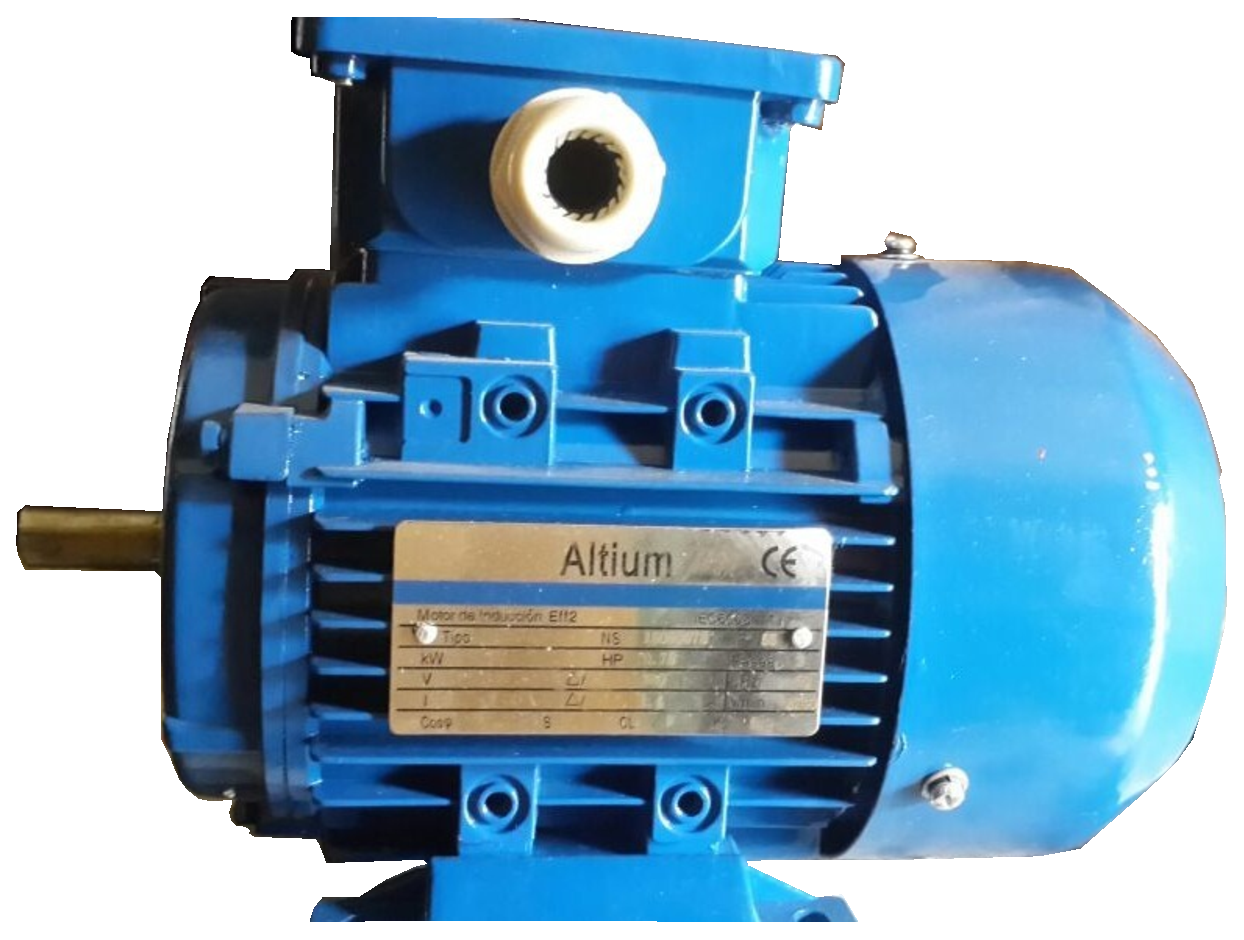
\includegraphics[scale=0.3]{motor.eps}}
	\captionof{figure}{Motor Altium}
	\label{fig:motor}

\end{minipage}

\subsection{Variador de velocidad}
\begin{tcolorbox}[colback=blue!5!white,colframe=blue!75!black,title=Variador de velocidad]
	Es utilizado para controlar la velocidad de giro de un motor.
	Para regular las revoluciones, se debe tener en cuenta las características del motor, ya que este tiene una curva propia de funcionamiento. Un variador es capaz de generar elementos control de aceleración, frenado, seguridad, control del torque y operaciones que mejoran la eficiencia energética.
\end{tcolorbox}

\subsubsection{Especificaciones}
El variador de velocidad que se utilizó pertenece a la marca \textbf{Schneider Electric} (Figura \ref{fig:variador}) y posee las siguientes características.
\paragraph*{Altivar 312}
\begin{minipage}[t]{.5\textwidth}
	\begin{itemize}
		\item 	Modelo: ATV312HU15N4
		\item   Tensión: 380-500 V
		\item 	Frecuencia: 50/60 Hz
		\item 	Potencia: 1.5kW / 2 HP
		\item 	Fases: 3
	\end{itemize}
\end{minipage}
\begin{minipage}[t]{.5\textwidth}
	\centering\raisebox{\dimexpr \topskip-\height}{%
		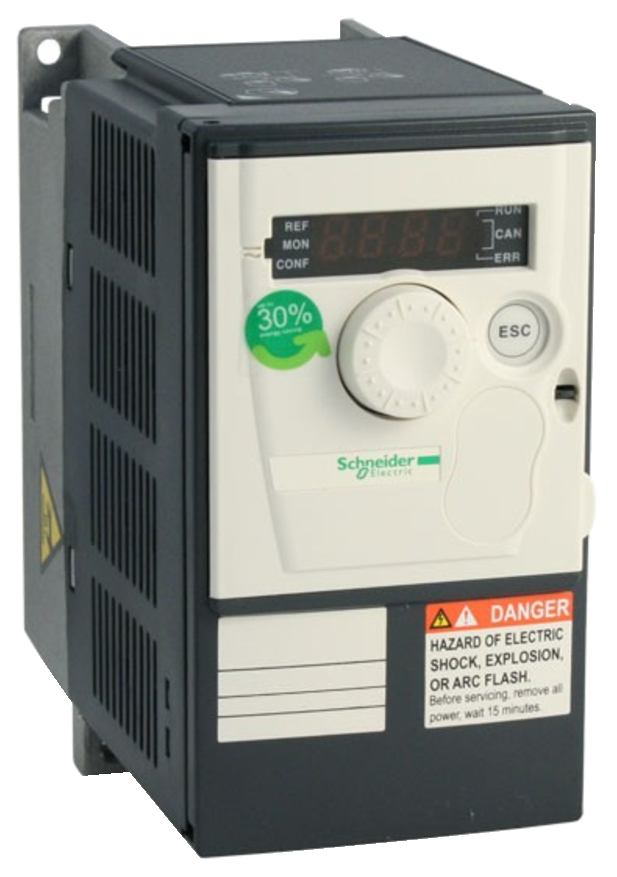
\includegraphics[scale=0.25]{variador.eps}}
	\captionof{figure}{Variador Altivar 312}
	\label{fig:variador}
\end{minipage}


Cabe destacar que el variador estima la velocidad de acuerdo a los parámetros del motor, por lo que para medir la velocidad verdadera se utiliza un tacómetro perteneciente al laboratorio.


\subsection{PLC}
\begin{tcolorbox}[colback=blue!5!white,colframe=blue!75!black,title=PLC]
	Es una computadora que se utiliza en la ingeniería de automatización para controlar procesos las industrias.
\end{tcolorbox}

\subsubsection{Módulos PLC M340}
El laboratorio cuenta con un PLC modular didáctico \ref{fig:didac} de la marca \textbf{Schneider Electric} de la familia \textbf{Modicon} modelo \textbf{M340} que posee los siguientes módulos:
\begin{itemize}
	\item BMX XBP 0400: bastidor para 4 módulos más la fuente de alimentación.
	\item BMX P34 2030: CPU 340-20 Ethernet CANopen.   (Comunicación)
	\item BMX ART 0414: 4 entradas TC/RTD con separación de potencial.
	\item BMX DDM 16022: 8 entradas digitales, y 8 salidas digitales por transistor PNP, todas ellas aisladas.
	\item BMX CPS 2000: Fuente de alimentación de 220V
\end{itemize}
\begin{center}
	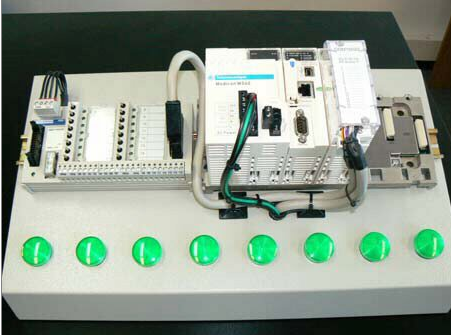
\includegraphics[scale=0.8]{educativo.png}
	\captionof{figure}{Módulo Didáctico PLC M340}
	\label{fig:didac}
\end{center}






\subsection{Banco de pruebas}
\subsection{Banco de pruebas}
\subsubsection{Elementos}
Se decidió que el banco de pruebas cuente con los siguientes elementos:
\begin{itemize}
	\item interruptor
	\item botón de marcha/ parada
	\item botón parada de emergencia
	\item señalización lumínica
	\item freno para generar perturbaciones 
	\item riel para colocar un nuevo motor que actuará como carga
	\item Panel de control
		\subitem Botón de emergencia
		\subitem Encendido/ apagado
		\subitem Potenciómetro para variar velocidad
		\subitem Display para observar velocidad
		\subitem Alarmas visuales
\end{itemize}
\subsubsection{Presupuesto--Valor--Costo a tal día}
\subsection{HMI}

Se realizó una interfaz humana maquina con los siguientes elementos:
	\begin{itemize}
		\item boton de start(acá o en el tablero???)
		\item varias velocidades configuradas previamente
		\item inversión y señalización del mismo
		\item torque???
		\item HMI
        	\subitem Alarmas
       		\subitem Información en tiempo real
        	\subitem Histórico de datos
        	\subitem Control general del banco
	\end{itemize}
	\begin{figure}[htb]
		\centering
		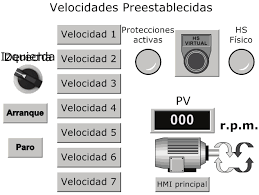
\includegraphics{HMIej.png}
		%\caption{Placa BME280}
		%\label{fig:BME280}
	\end{figure}

\newpage
\section{Preliminares}

\subsection{Programación variador de velocidad}


Para realizar la configuración del variador de velocidad con los parámetros del motor se utilizó el software SoMove a través del protocolo ModBus. Se descargó la ultima versión desde la página oficial de Schneider\footnote{\url{https://www.se.com/ar/es/product-range-presentation/2714-somove/}} y luego, la librería DTM correspondiente al variador a utilizado \footnote{\url{https://www.se.com/ar/es/download/document/Altivar_DTM_Library/}}.

Una vez realizado esto se procedió a generar un nuevo proyecto donde se eligió las características del variador (Figura \ref{fig:so1} y \ref{fig:so2}). El próximo paso fue realizar por medio del software la carga de los parámetros del motor (Figura \ref{fig:paramsomove}) y establecer el modo de funcionamiento de las entradas y el protocolo de comunicación.
\begin{figure}[h]
	\centering
	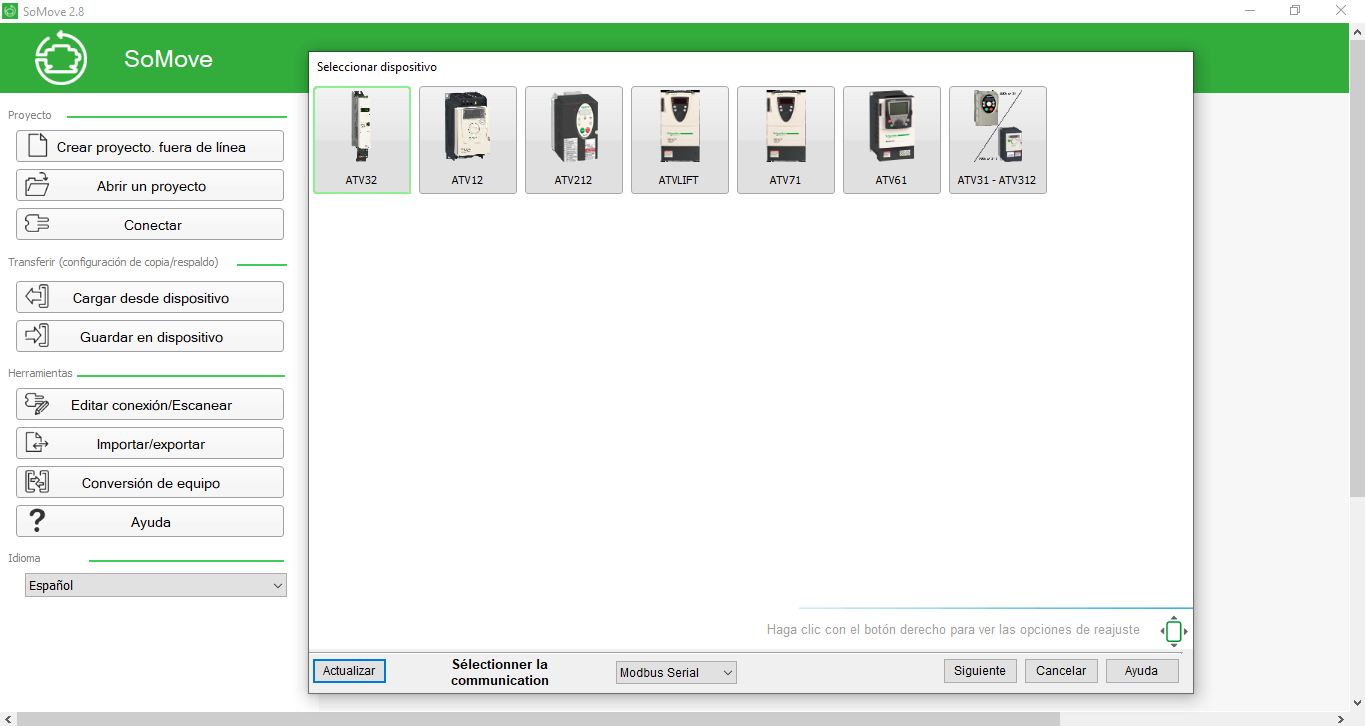
\includegraphics[width=0.9\linewidth]{somove1.png}
	\captionof{figure}{Elección de Altivar 312}
	\label{fig:so1}
\end{figure}
\begin{figure}[H]
	\centering
	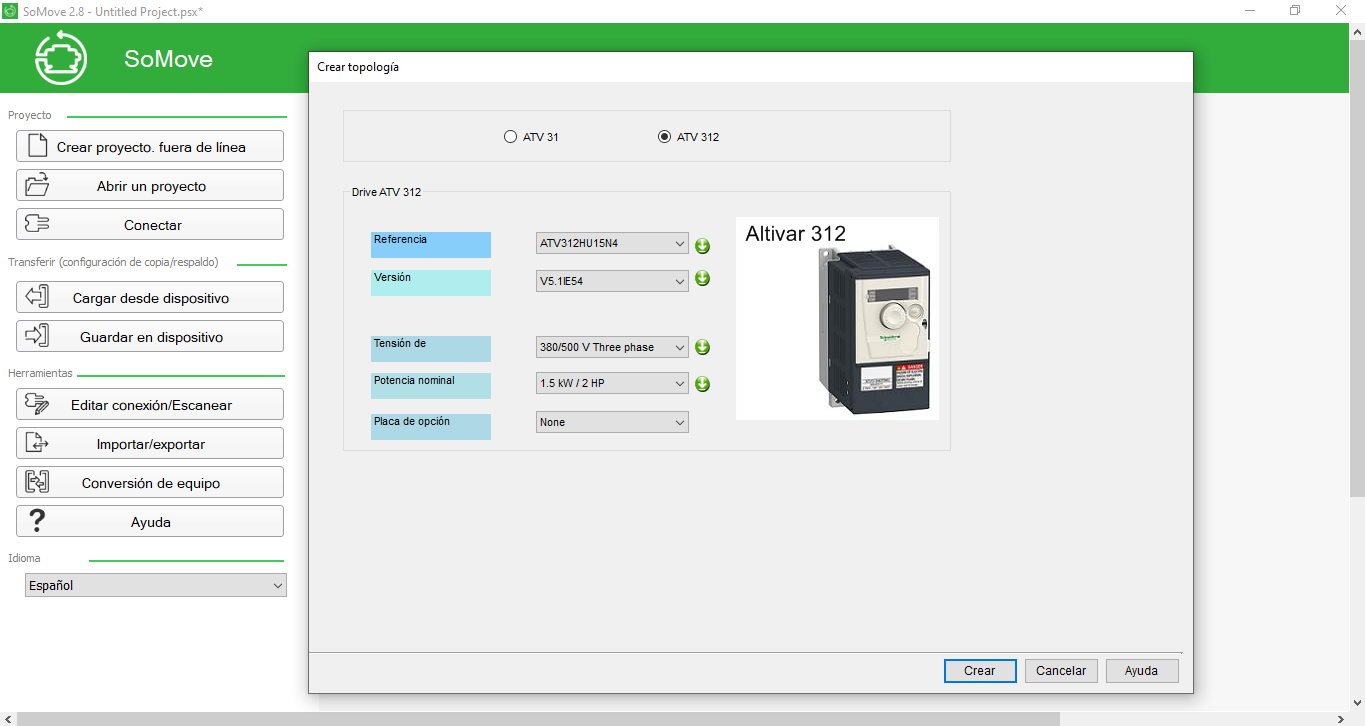
\includegraphics[width=0.9\linewidth]{somove2.png}
	\captionof{figure}{Parámetros del variador}
	\label{fig:so2}
\end{figure}

\begin{figure}[H]
	\centering
	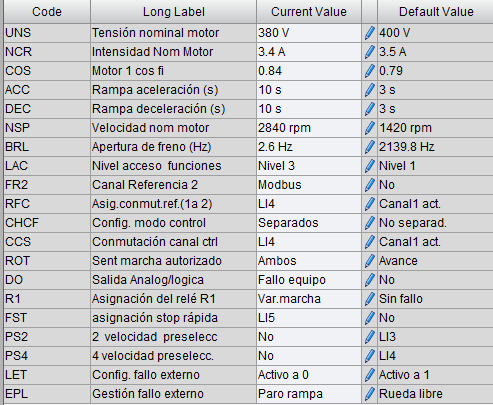
\includegraphics[width=0.9\linewidth]{images/paramsomove}
	\captionof{figure}{Lista de parámetros modificados}
	\label{fig:paramsomove}
\end{figure}


Para realizar esta primera configuración se realizó la comunicación de la computadora con el variador a través del protocolo \textbf{Modbus} (Figura\ref{fig:pcvar}) por medio de un cable que en un extremo poseía una ficha RJ45 con un conversor RS485 y en el otro, ficha USB (Figura \ref{fig:paramsomove1}). 
\begin{figure}[H]
	\centering
	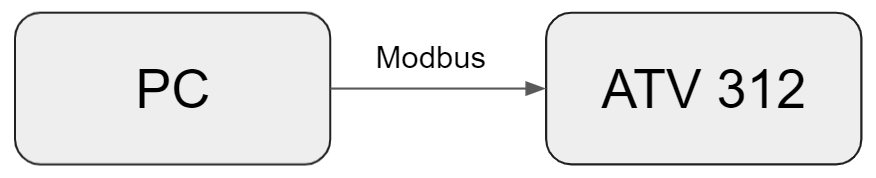
\includegraphics[width=0.7\linewidth]{pc_var.png}
	\captionof{figure}{Diegrama comunicación PC- Variador}
	\label{fig:pcvar}
\end{figure}

\begin{figure}[H]
	\centering
	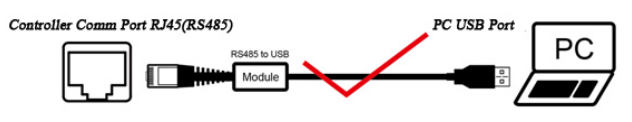
\includegraphics[width=0.9\linewidth]{paramsomove1.png}
	\captionof{figure}{Cable de comunicación}
	\label{fig:paramsomove1}
\end{figure}


\subsection{Comunicación variador de velocidad - PLC}
Para poder realizar la comunicación entre el variador y el PLC es necesario contar con un cable que realice la conexión desde la salida CANOpen a RS485, para esto se necesitó hacer un cable con las fichas correspondientes en cada extremo según las conexiones que muestran en la Figura \ref{fig:cable}, colocando a su vez resistencia de 120 $\Omega$ en cada punta para evitar ruidos eléctricos y fenómenos de reflexión en la línea.

\begin{figure}[htbp]
    \centering
    \subfigure[Ficha entrada/salida variador]{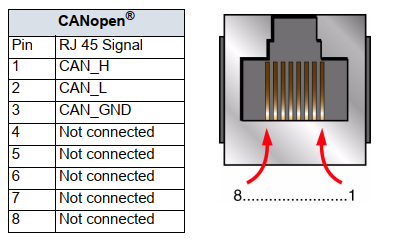
\includegraphics[width=60mm]{canconectores.png}}
    \subfigure[Ficha entrada/salida PLC]{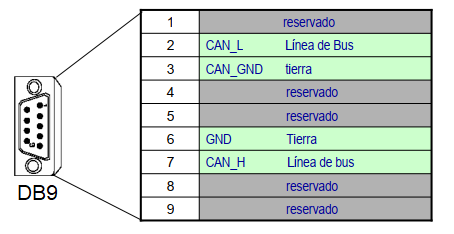
\includegraphics[width=80mm]{candb9.png}}
    \caption{Conexión fichas RJ45- DB9} \label{fig:cable}
    \end{figure}



\subsection{Programación Unity Pro}


Para generar la base del proyecto para trabajar, se debe descargar desde la página oficial e instalar el software Unity Pro XL y la librería DTM utilizada en el software soMove correspondiente al variador que se posee. Una vez que esto está instalado se abre un nuevo proyecto y se configura siguiendo los siguientes pasos.
\begin{enumerate}
	\item Se selecciona el bastidor que se posee.
	\item En la configuración gráfica del bastidor (Figura \ref{fig:uni0})
	podemos introducir los módulos
	deseados haciendo un clic en la
	posición seleccionada (Figura \ref{fig:uni1}).
	El laboratorio cuenta con un PLC modular didáctico de la marca \textbf{Schneider Electric} de la familia \textbf{Modicon} modelo \textbf{M340} con los módulos nombrados anteriormente (Sección \ref{sec:didac}). 
	\item Se debe configurar el módulo Ethernet desde el explorador de
	Proyectos desplegamos la
	carpeta Comunicación y se realiza clic con el botón derecho sobre Redes y luego en Nueva Red, Ethernet (Figura  \ref{fig:inter}).
	\item Se creó una nueva sección para lenguaje FDB para ver parámetros básicos.
	\begin{itemize}
		\item Los Diagramas de Bloques de Función consisten en un Editor gráfico orientado al dibujo
		de bloques. El lenguaje consiste en los Bloques de Funciones reusables elementales y
		derivados.
	\end{itemize}
%\item Para realizar la conexión del PLC con la computadora se utiliza protocolo TCP/IP a través de la dirección 192.168.10.187 (Dirección que el PLC tiene configurada internamente)(Figura \ref{fig:direcc}) y (Figura \ref{fig:inter})
\end{enumerate}
	
	\begin{comment}
	que posee los siguientes módulos:
\begin{itemize}
\item BMX XBP 0400: bastidor para 4 módulos más la fuente de alimentación.
\item BMX P34 2030: CPU 340-20 Ethernet CANopen.   (Comunicación)
\item BMX ART 0414: 4 entradas TC/RTD con separación de potencial.
\item BMX DDM 16022: 8 entradas digitales, y 8 salidas digitales por transistor PNP, todas ellas aisladas.
\item BMX CPS 2000: Fuente de alimentación de 220V
\end{itemize}

	\end{comment}


\begin{center}
	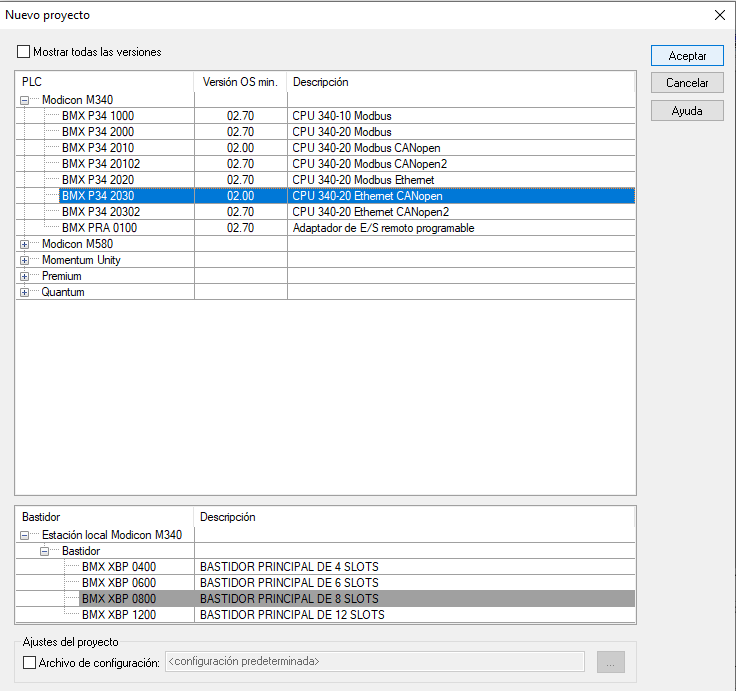
\includegraphics[width=0.9\linewidth]{unit1.png}
	\captionof{figure}{Elección del bastidor}
	\label{fig:uni1}
	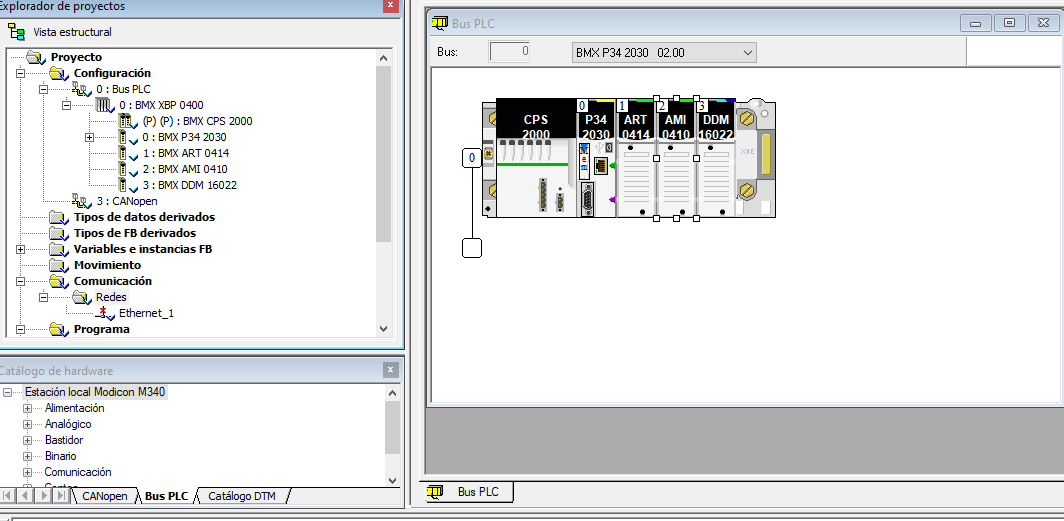
\includegraphics[width=0.9\linewidth]{unity1.png}
	\captionof{figure}{Módulos PLC}
	\label{fig:uni0}
\end{center}

\begin{figure}[h]
	\centering
	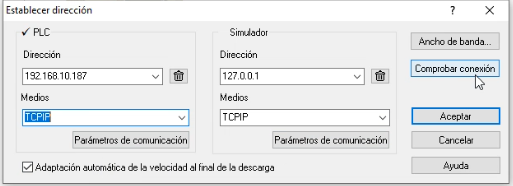
\includegraphics[scale=1]{1.direcc.png}
	\captionof{figure}{Dirección IP}
	\label{fig:direcc}
\end{figure}


\begin{figure}[h]
	\centering
	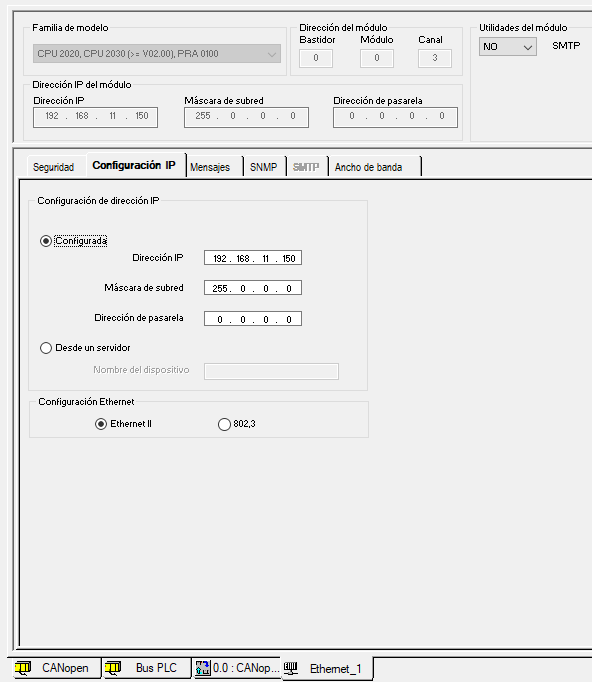
\includegraphics[width=0.9\linewidth]{2.ethern.png}
	\captionof{figure}{Dirección módulo Ethernet}
	\label{fig:inter}
\end{figure}

Una vez que se completó la configuración de la comunicación variador - PLC se procedió a crear una \textit{Pantalla de operador} dentro del mismo programa (Figura \ref{fig:previo})
la cual fue utilizada para interactuar y observar diversos parámetros, como modificar velocidades, observar señales luminosas y ver distintos valores proporcionados por el variador de velocidad.
 
\begin{figure}[H]
	\centering
	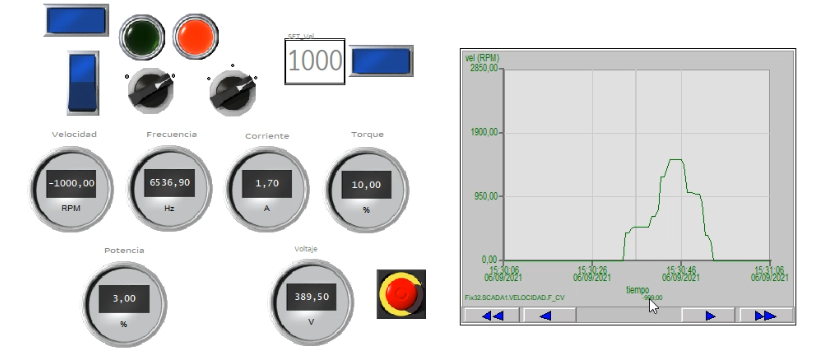
\includegraphics[width=0.9\linewidth]{3.previo.png}
	\captionof{figure}{HMI simple}
	\label{fig:previo}
\end{figure}

Para realizar la programación del HMI se utilizó los bloques de funciones de movimiento (Motion Function Block, MFB) del software UnityPro (Figura \ref{fig:read}). Estos bloques necesitan de un bloque maestro ``CAN\_HANDLER'' el cual permite comprobar la comunicación CANopen, así como la coherencia
entre las configuraciones de software y física.
\\
Otros de los bloques más utilizados dentro del programa fueron ``MC\_READPARAMETER'' que se utiliza para leer, mediante mensajes Service Data Object
(SDO), una variable del variador definida en una dirección CANOpen dada por el fabricante \cite{ComManual}.

\begin{figure}[H]
	\centering
	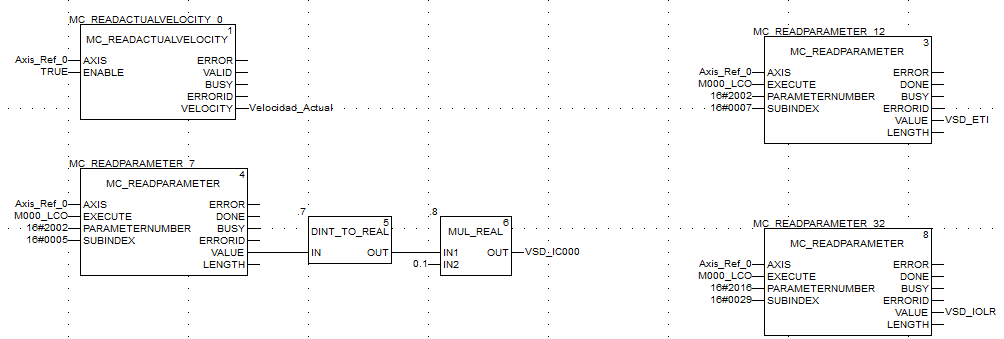
\includegraphics[width=0.9\linewidth]{4.read.png}
	\captionof{figure}{Programa con bloques MFB}
	\label{fig:read}
\end{figure}



\subsubsection{Entradas analógicas}
En el rack del PLC se encuentra un módulo AMI0410 el cual consiste en cuatro entradas analógicas (Tensión/Corriente) aisladas del siguiente tipo:
\begin{itemize}
	\item Corriente +/- 20 mA
\item 	Corriente 0 a 20 mA
\item 	Corriente 4 a 20 mA
\item 	Tensión +/- 10 V
\item 	Tensión +/- 5 V
\item 	Tensión 0 a 10 V
\item 	Tensión 0 a 5 V
\item 	Tensión 1 a 5 V
	
\end{itemize}

El módulo dispone de 20 bornes accesibles al usuario siendo el diagrama de conexión tanto para entradas de tensión o corriente el mostrado en la figura \ref{fig:modulo}.

Para la configuración en Unity PRO se eligen de las opciones anteriores la que se va a utilizar, en nuestro caso de 4 a 20 mA y el escalado predefinido de fábrica es de 0 a 10000 cuentas pero modificable por el usuario entre -32768 a 32767 ya que la resolución de las entradas analógicas es de 16 bit. También es posible añadir un filtro de primer orden a cada entrada por software (Figura \ref{fig:param}).

Con el rango de cuentas del módulo determinado, se requiere escalar la variable para obtener el valor físico y así utilizarla para la visualización y control del banco de pruebas.
Para el escalado de la señal de entrada se realizó un nuevo bloque FB derivado, que fue construido en base a elementos primarios, para evitar realizar un proceso repetitivo para el escalado de varias señales (Figura \ref{fig:escalado}).

En la variable de entrada se coloca la señal que se desea escalar. En los límites de entrada se escribe el rango del módulo visto anteriormente, y en los límites de salida, los escalados obtenidos del instrumento utilizado. A la salida del bloque se obtiene el valor físico visualizado o transmitido por el instrumento.

\begin{figure}[H]
	\centering
	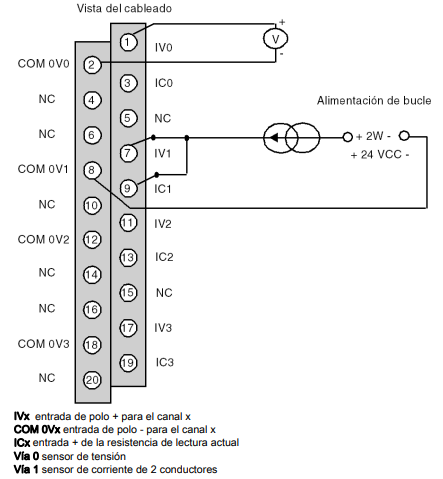
\includegraphics[width=0.6\linewidth]{modulo.png}
	\captionof{figure}{Módulo AMI0410}
	\label{fig:modulo}
\end{figure}
\begin{figure}[H]
	\centering
	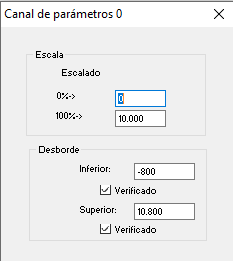
\includegraphics[width=0.9\linewidth]{param.png}
	\captionof{figure}{Rango y escalado}
	\label{fig:param}
\end{figure}

\begin{figure}[H]
	\centering
	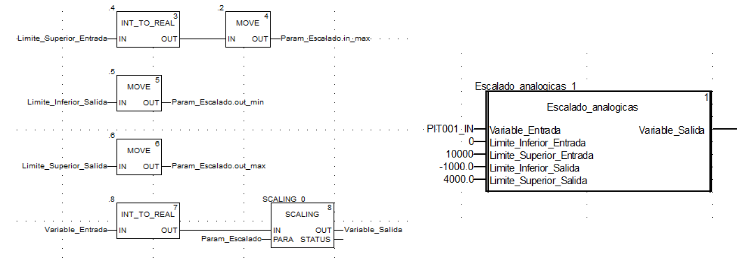
\includegraphics[width=0.9\linewidth]{escalado.png}
	\captionof{figure}{Bloques de escalado}
	\label{fig:escalado}
\end{figure}


\subsubsection{Entradas analogicas para termocuplas o detectores de temperatura resistivos (RTD)}
Se utiliza el módulo ART0414 que consiste en cuatro entradas aisladas en las que se pueden conectar sensores de temperatura del tipo termocupla y RTD con las siguientes características:
\begin{itemize}
	\item RTD IEC Pt100/Pt1000, US/JIS Pt100/Pt1000, Cu10, Cu50, Cu100, Ni100/Ni1000 en 2, 3 o 4 conductores
	\item Termoelemento del tipo B, E, J, K, L, N, R, S, T, U
\item 	Tensión $+/-$ 40 mV a 1,28 V
	
\end{itemize}

Para la conexión de sensores se utiliza el accesorio TELEFAST ABE-7CPA412 (Figura \ref{fig:ABE}). Y se tienen las siguientes formas de conexión dependiendo el tipo de sensor (Figura \ref{fig:ABE2}).

\begin{figure}[H]
	\centering
	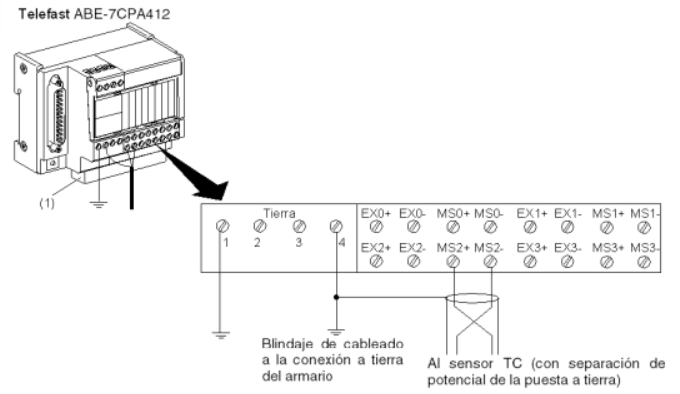
\includegraphics[width=0.9\linewidth]{ABE.png}
	\captionof{figure}{Accesorio TELEFAST ABE-7CPA412}
	\label{fig:ABE}
\end{figure}
\begin{figure}[H]
	\centering
	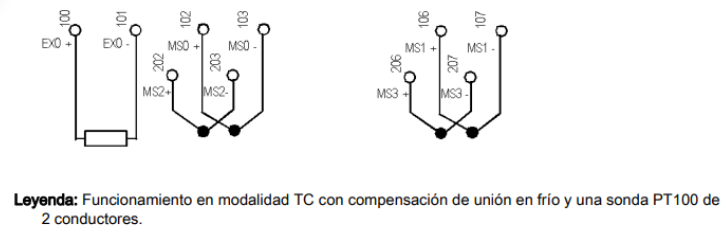
\includegraphics[width=0.9\linewidth]{ABE2.png}
	\captionof{figure}{Conexión según sensor}
	\label{fig:ABE2}
\end{figure}

Para su configuración en Unity Pro se selecciona en Rango las características del sensor y en escala se modifica los valores para que coincidan con los máximos y mínimos del sensor. Para el caso de RTD y Termocupla los valores son múltiplos de 10 respecto a la temperatura en °C o °F. 
En la imagen \ref{fig:ABE3} se observan dos elementos ya que se probó realizar la configuración con una termocupla y un RTD. Finalmente se eligió el RTD PT1000 dónde el valor obtenido se divide por 10 y se genera el valor de temperatura en °C con un decimal  (Figura \ref{fig:ABE3}).

\begin{figure}[H]
	\centering
	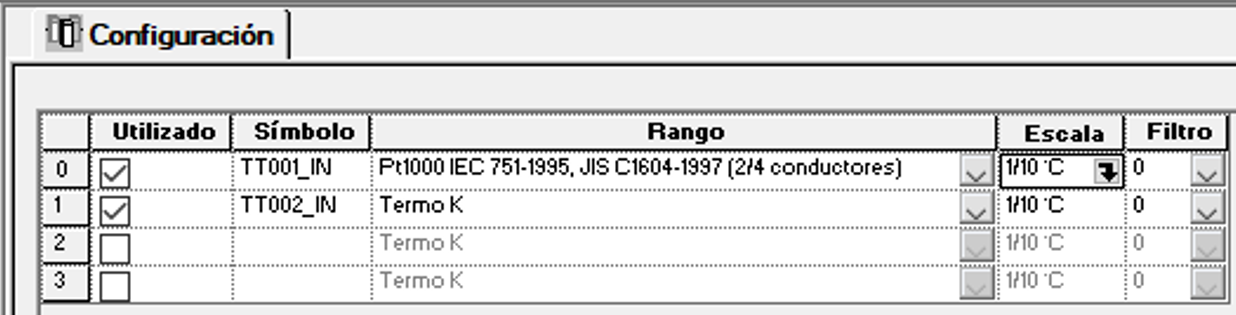
\includegraphics[width=0.9\linewidth]{ABE3.png}
	\captionof{figure}{Rango y escalado}
	\label{fig:ABE3}
\end{figure}

\begin{figure}[H]
	\centering
	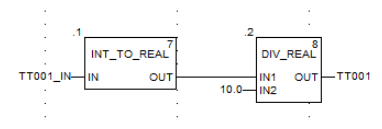
\includegraphics[width=0.6\linewidth]{ABE4.png}
	\captionof{figure}{Bloque de escalado}
	\label{fig:ABE4}
\end{figure}

\subsubsection{Medición de caudal}
Según la cantidad de flujo que pase por el caudalímetro, este entregaría pulsos que debían ser leídos con un módulo externo del PLC por la baja resolución que posee. Para esto se planteó utilizar un ESP8266 como interfaz para obtener los pulsos, colocarlos en un registro y enviarlos por un servidor Modbus TCP cada 20ms al PLC. En la sección de programación del PLC se realizó las cuentas correspondientes para realizar la conversión de pulsos a caudal (Figura \ref{fig:modtcp}). Tanto para el módulo, como para el caudalímetro se usó una fuente externa de 3,3 V de alimentación.
\begin{figure}[htbp]
	\centering
	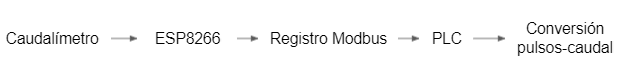
\includegraphics[scale=1]{esp_mod.png}
	\captionof{figure}{Diagrama de flujo del caudalimetro} 
	\label{fig:modtcp}
\end{figure}
\newpage

%\url{
%https://download.schneider-electric.com/files?p_enDocType=User+guide&p_File_Name=35010608_K01_000_11.pdf&p_Doc_Ref=35010608K01000}

	
\section{Desarrollo}


A partir de lo programado en Unity PRO utilizado para obtener los primeros registros, se realizó modificaciones necesarias donde se eliminó y agregó variables de la lista de direcciones (Tabla {\ref{tab:direc} en Anexo \ref{Anexo1}) que se creyeron necesarias a la hora de implementar el proyecto quedando un mapa de memoria como el de la figura \ref{fig:memoria}
\begin{figure}[h!]
	\centering
	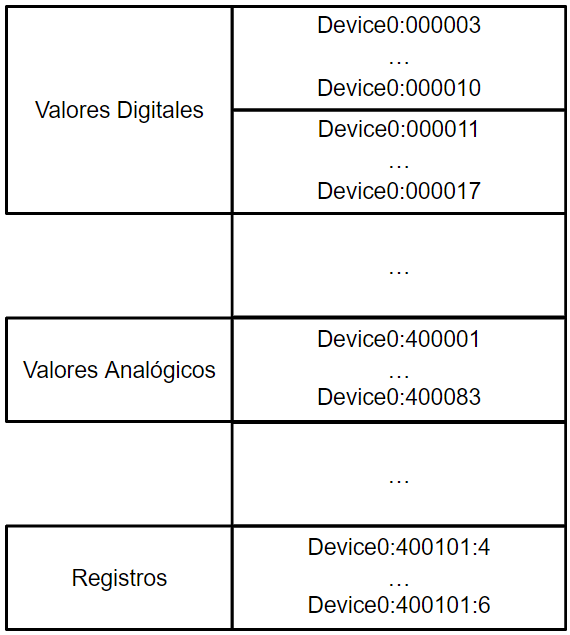
\includegraphics[scale=0.6]{memoria.png}
	\captionof{figure}{Esquema de memoria}
	\label{fig:memoria}
\end{figure}


\subsection{Adquisición de datos}
En el objetivo se propuso que el sistema sea capaz de controlar presión o caudal. Para lograr lo estipulado, como en cualquier sistema de control, es necesario conocer las plantas con las que se trabajará, reconociendo en el banco de pruebas tres sistemas con los que se trabajará:
\begin{itemize}
	\item PIT01: Presión 1 medida a la salida de la bomba.
	\item PIT02: Presión 2 medida luego de la columna que deriva el fluido.
	\item FT01: Caudal que pasa por PIT02.
\end{itemize}
Para realizar las estimaciones de las plantas del sistema se utilizó el protocolo OPC en conjunto con Matlab. Por medio de OFS, se procedió a crear y configurar un servidor con la dirección correspondiente y se seleccionó el programa realizado en UnityPro donde se encontraban las variables necesarias (Figura \ref{fig:opc1}).

\begin{figure}[htbp]
	\centering
	\subfigure[]{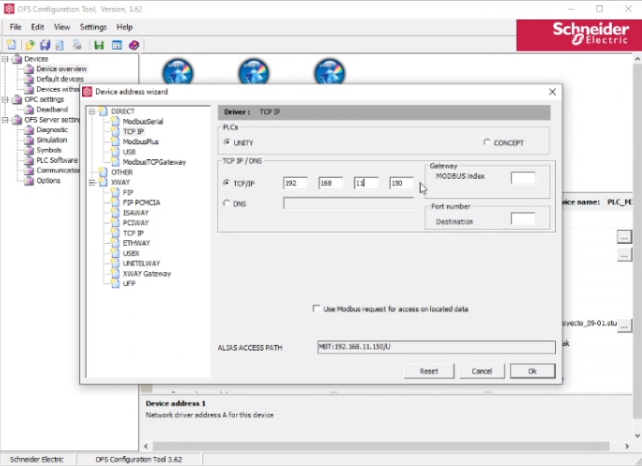
\includegraphics[width=70mm]{ofs1.png}}
	\subfigure[]{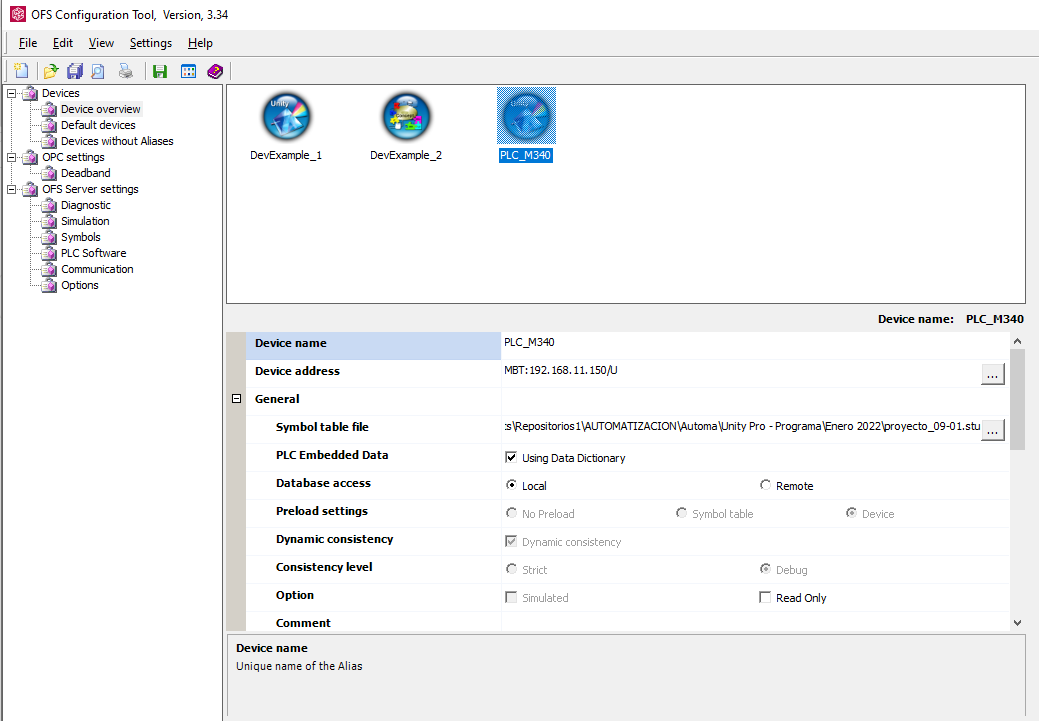
\includegraphics[width=70mm]{ofs2.png}}
	\caption{Configuración OPC} \label{fig:opc1}
\end{figure}


Una vez configurado el servidor se abre el programa \textbf{OPC Factory Server} dando inicio al servidor (Figura \ref{fig:opc2}a). Para observar si la comunicación esta establecida de forma correcta, se utilizó el programa \textbf{OFS Client} dónde se debió agregar el tag correspondiente a la variable a observar (Figura \ref{fig:opc2}b)

\begin{figure}[htbp]
	\centering
	\subfigure[OPC Factory Server]{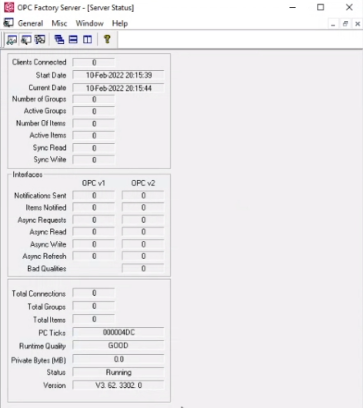
\includegraphics[width=40mm]{ofs3.png}}
	\subfigure[OFS Client]{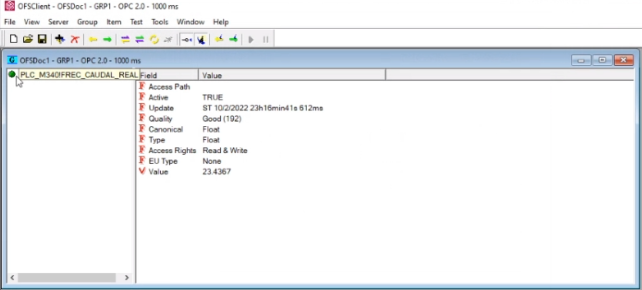
\includegraphics[width=80mm]{ofs4.png}}
	\caption{Conexión servidor OPC} \label{fig:opc2}
\end{figure}

Una vez corroborada la comunicación con el servidor OPC, se procedió a crear un cliente OPC en Simulink (perteneciente a Matlab) para adquirir y guardar las variables necesarias. 


\subsubsection{Uso de Matlab}
En el entorno Simulink se procedió a configurar un bloque de cliente OPC con la dirección IP donde se encuentra el servidor previamente creado. Luego, para leer las variables necesarias se creó un bloque de lectura OPC (Figura \ref{fig:opcsimu} a) y con un bloque \textit{Scope}, se activó la opción para que se guarden los vectores de las variables a estudiar (Figura \ref{fig:opcsimu} b). 


\begin{figure}[htbp]
	\centering
	\subfigure[]{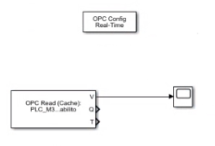
\includegraphics[width=60mm]{ofs5.png}}
	\subfigure[]{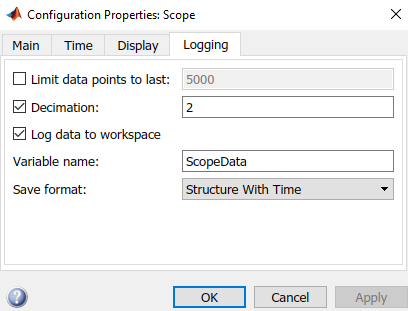
\includegraphics[width=60mm]{ofs6.png}}
	\caption{Cliente OPC en Simulink} \label{fig:opcsimu}
\end{figure}



\subsubsection{Estimación de la planta}
Para realizar la estimación de las plantas se utilizó el Método de Strejc con retardo (Figura \ref{fig:norden})\cite{pomares2011sistemas}.
Este método se emplea para la identificación de sistemas de polos múltiples,
mediante los parámetros Tu y Ta obtenidos sobre la respuesta del sistema.
Tras obtener el valor de los parámetros, se determinará la multiplicidad del polo. 
\begin{figure}[htb]
	\centering
	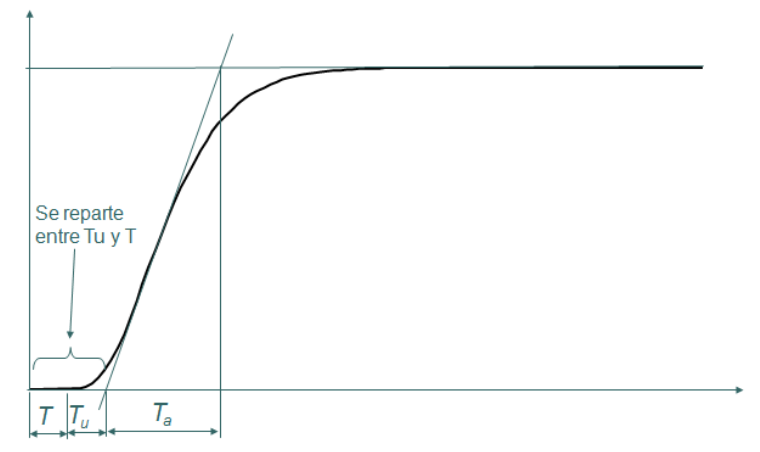
\includegraphics[width=0.9\linewidth]{norden.png}
	\captionof{figure}{Parámetros de Strejc con retardo}
	\label{fig:norden}
\end{figure}

La función de transferencia general para un sistema de polos múltiples es:
\begin{equation}
	G(s)\;=\;\frac K{(1\;+\;\tau\;.\;s)^n}\;.\;e^{-T.s}
\end{equation}
Dónde:
\begin{itemize}
	\item K:  Ganancia del sistema $K = \frac{\triangle y}{\triangle u}$
	\item $\tau$: constante de tiempo
	\item T= Retardo
\end{itemize}
Para obtener la función de transferencia se realizó un script en Matlab que dió como resultado los siguientes sistemas:
\begin{itemize}
	\item Planta de presión PIT01:
	\begin{equation}
	 G(s)\;=\;\frac {0,135}{(1\;+\;1,3783\;.\;s)^3}\;.\;e^{-1,2.s}
	\end{equation}
	\item Planta de presión PIT02: 	
	\begin{equation}
		G(s)\;=\;\frac {0,125}{(1\;+\;1,054\;.\;s)^3}\;.\;e^{-s}
	\end{equation}
	\item Planta de caudal FT01:
		\begin{equation}
		G(s)\;=\;\frac {0,003784}{(1\;+\;0,7027\;.\;s)^3}\;.\;e^{-s}
	\end{equation}
\end{itemize}

\paragraph{Comparación numérica- real}
En las siguientes imágenes (Figura \ref{fig:PIT01} ,\ref{fig:PIT02} y \ref{fig:FT01}) se observa la gráfica de cada planta estimada comparada con los datos obtenidos en las mediciones.
\begin{comment}
$C:\Users\glori\Desktop\DANIELA\VISUAL_DANI\Automa\MATLAB\Prueba_PLANTA\Imaagenes Calculo Plantas\FIT001
Strenj_RESPUESTA.png$
\end{comment}

Cabe destacar que las plantas fueron calculadas para los rangos medios que normalmente se utilizará dado que los sistemas de presiones no presentan una ganancia estática constante.
Se puede observar que los sistemas de tercer orden se adaptan bien a los datos obtenidos durante las pruebas.
\begin{comment}
no borrar opr las dudas que quisimos poner esto
 
 dónde el motor no era esforzado a calentarse ni la bomba era sobreexigida

escalones ubicados en la parte central del rango útil estipulado .

 además obtener un control apropiado al sistema: algo no muy rapido ni muy lento
\end{comment}


\begin{figure}[htb]
	\centering
	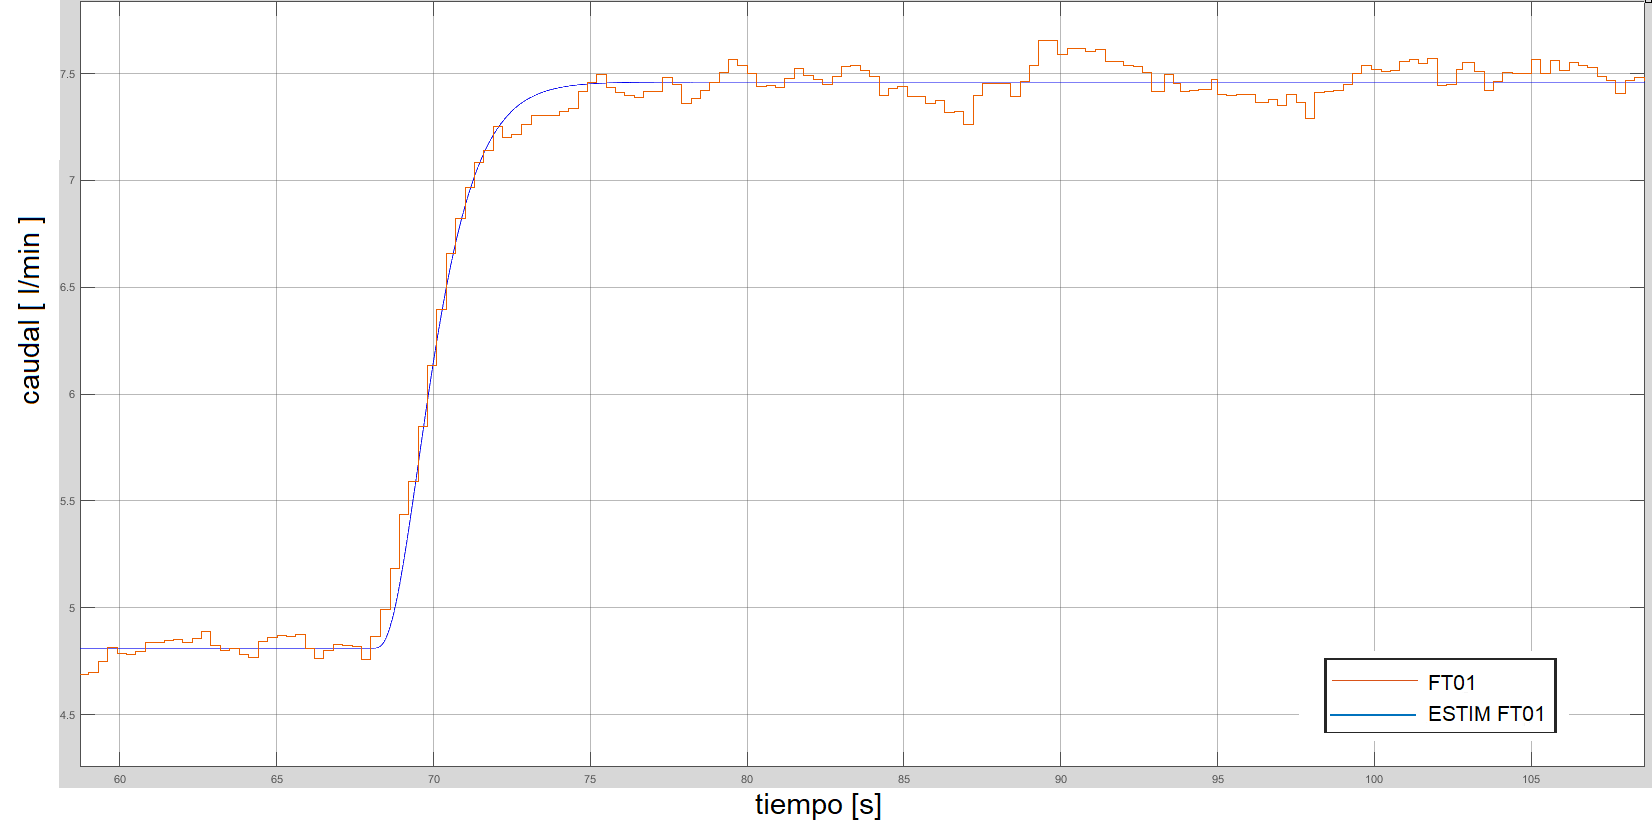
\includegraphics[width=0.8\linewidth]{Strenj_RESPUESTA.png}
	\captionof{figure}{Comparación de la planta estimada y los valores obtenidos para FT01}
	\label{fig:FT01}
\end{figure}
\begin{figure}[htb]
	\centering
	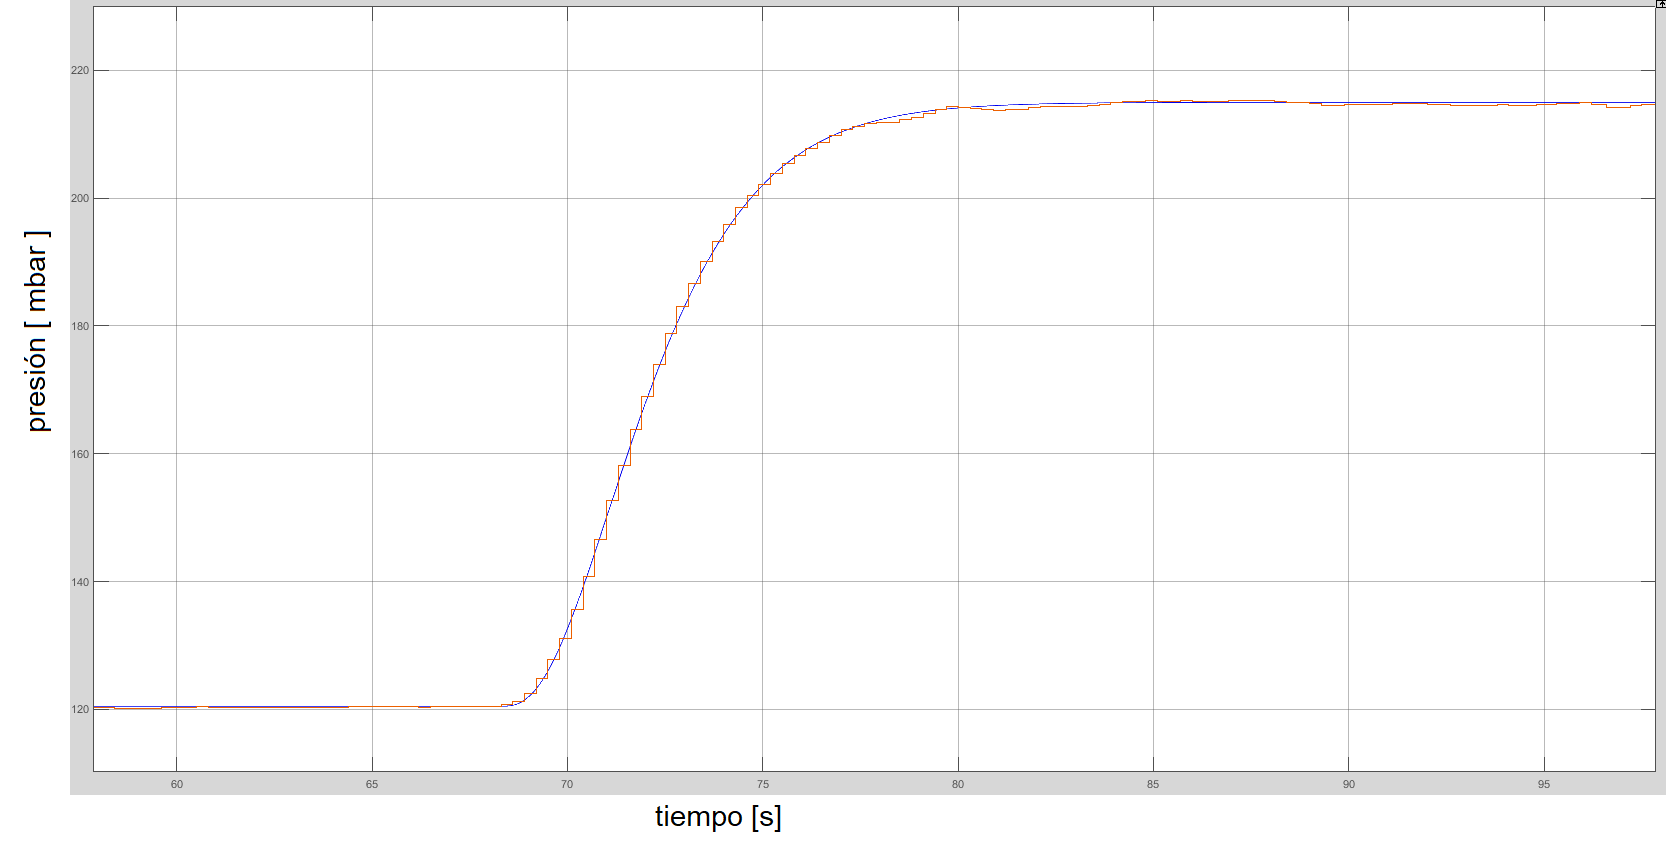
\includegraphics[width=0.8\linewidth]{Strenj_RESPUESTA1.png}
	\captionof{figure}{Comparación de la planta estimada y los valores obtenidos para PIT01}
	\label{fig:PIT01}
\end{figure}




\begin{figure}[htb]
	\centering
	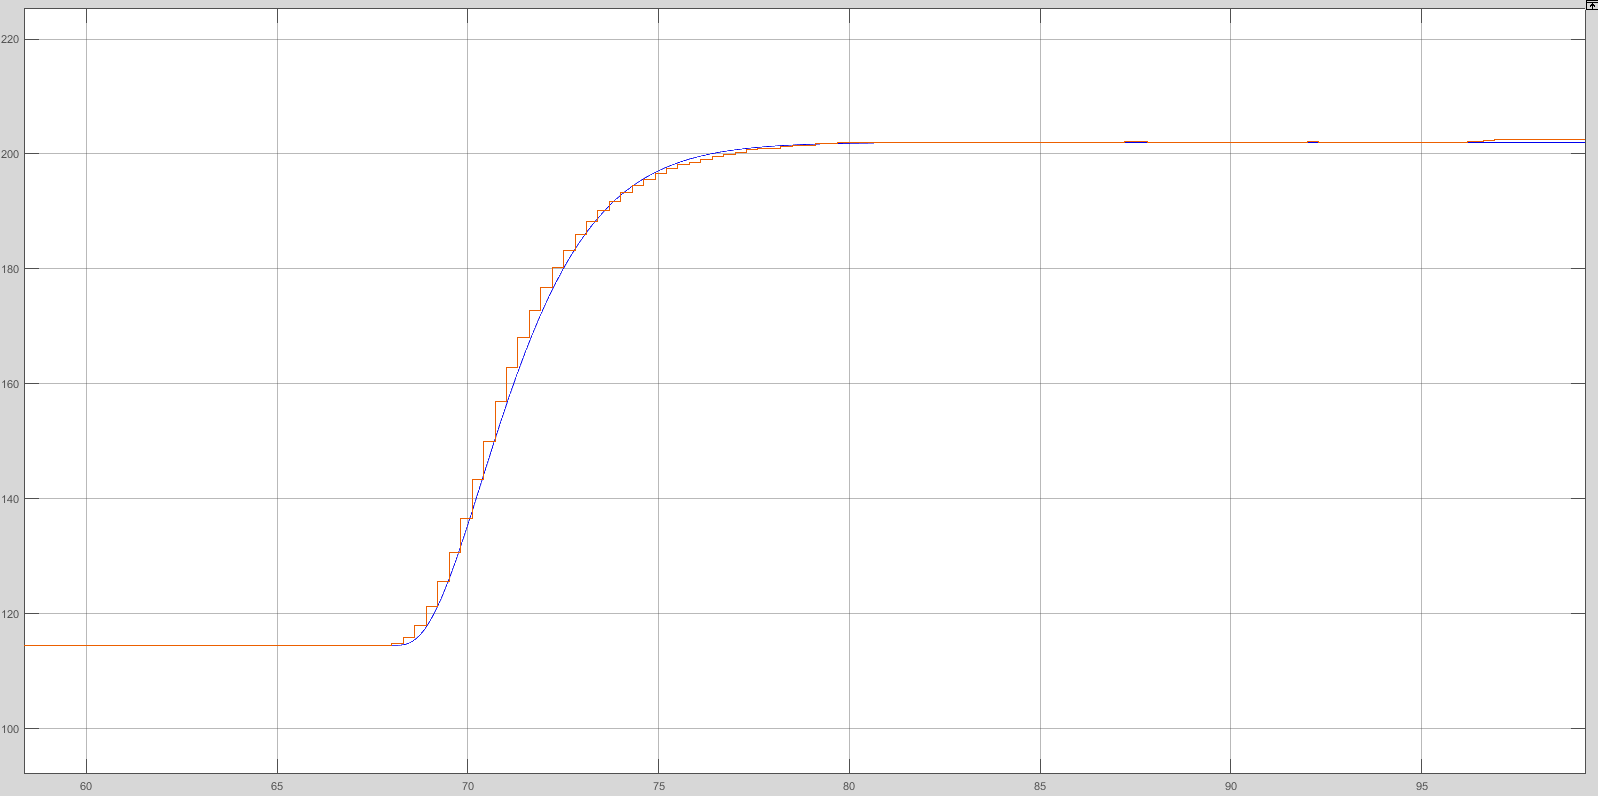
\includegraphics[width=0.8\linewidth]{Strenj_respuesta2.png}
	\captionof{figure}{Comparación de la planta estimada y los valores obtenidos para PIT02}
	\label{fig:PIT02}
\end{figure}






\subsubsection{Cálculo del controlador PID}
El controlador PID de cada planta se calculó con \textit{Tune PID controllers} (Figura \ref{fig:PIDcontr}), dónde se buscó que las respuestas sean capaces de mitigar los cambios producidos por la ganancia, y además obtener un control apropiado al sistema. \\
Se realizaron pruebas con diversos PID para observar la respuesta a cada sistema, en las figuras \ref{fig:FT1} , \ref{fig:PIT1} y \ref{fig:PIT2} se comparan dos PI para cada planta. Se observan que las respuestas se buscaron que no sean tan rápidas ni con tanto sobre paso.

Los valores obtenidos de la aplicación perteneciente a Matlab se muestran en la tabla \ref{tab:pid}, los cuales se ingresaron en los bloques de \textit{UnityPro} con las respectivas modificaciones numéricas según lo establecido por el software. Los valores mostrados en dicha tabla serán usados al momento de restablecer los PID del sistema en la pantalla SCADA presionando el botón C (Figura \ref{fig:LCs}).
\begin{figure}[h!]
	\centering
	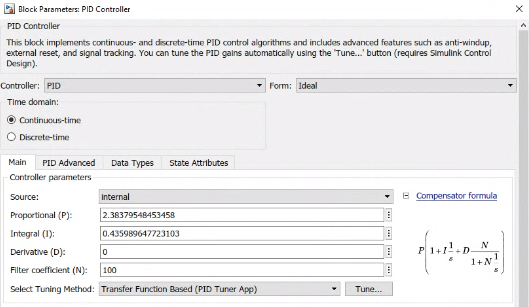
\includegraphics[scale=0.7]{pidmatlab.png}
	\captionof{figure}{PID Controller}
	\label{fig:PIDcontr}
\end{figure}

\begin{figure}[h!]
	\centering
	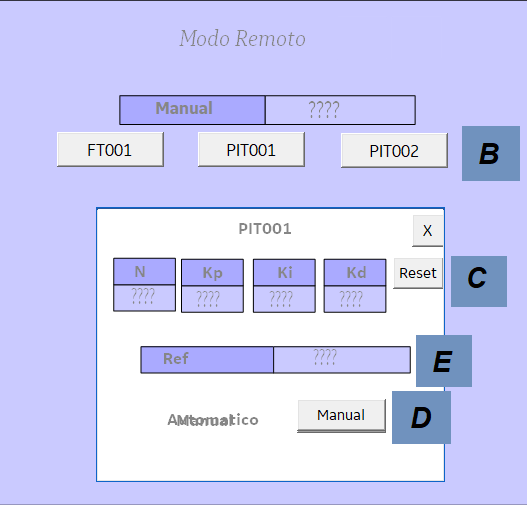
\includegraphics[width=60mm]{p_4a.png}
	\captionof{figure}{Modo lazo cerrado}
	\label{fig:LCs}
\end{figure}

\begin{comment}
Se observa que algunos de los controladores PID son del tipo proporcional integrador, dando así ya que la ganancia en los diferentes escalones en la planta no era constante. Al utilizar un PI genera una salida con error de estado estacionario cero. 
\end{comment}

\begin{table}[h]
	\centering
	\begin{tabular}{|l|l|l|l|}
		\hline
		& PIT01 & PIT02 & FT01 \\ \hline
		$K_p$ & 3,11 & 3,36 & 117,1 \\ \hline
		$K_i$ & 0,35 & 0,46 & 0,62 \\ \hline
		$K_d$ & 0 & 0 & 0 \\ \hline
		N & 100 & 100 & 100 \\ \hline
	\end{tabular}
	\captionof{table}{Valores de PID}
	\label{tab:pid}
\end{table}

\begin{comment}
	C:\Users\glori\Desktop\DANIELA\VISUAL_DANI\Automa\MATLAB\22-05\Comparacion PID y PLANTAS\FT01
	Respuesta_Strenj
\end{comment}






\begin{figure}[htbp]
	\centering
	\subfigure[]{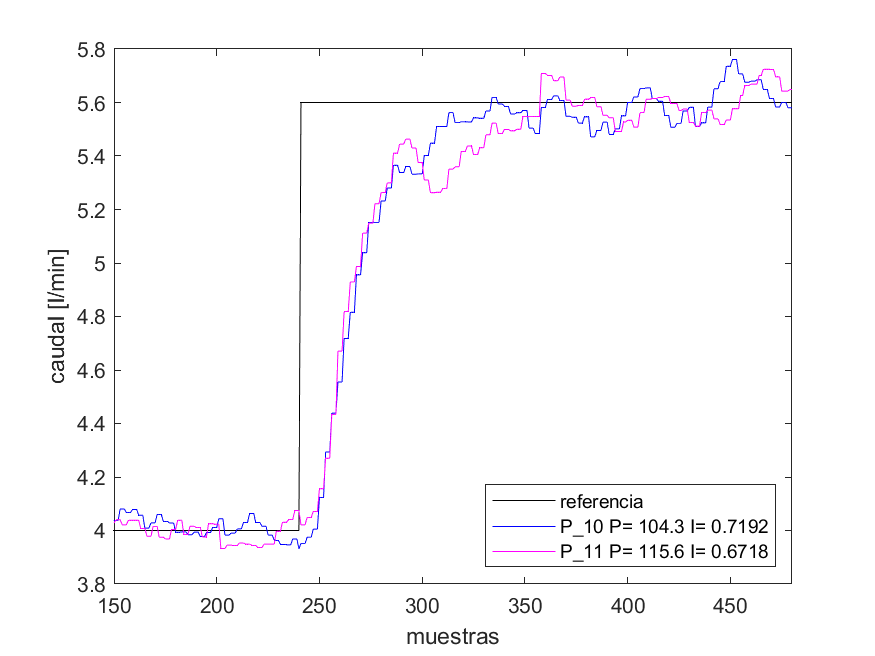
\includegraphics[width=80mm]{FT1b.png}}
\hspace{-4mm}
	\subfigure[]{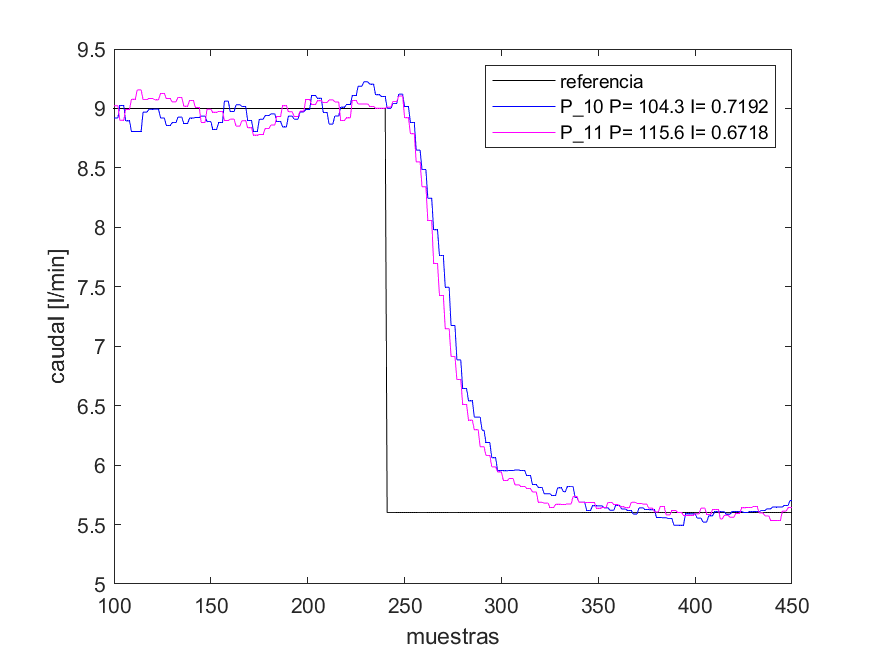
\includegraphics[width=80mm]{FT1c.png}}
	\caption{Comparación PID para FT01} \label{fig:FT1}
\end{figure}

\begin{figure}[htbp]
	\centering
	\subfigure[]{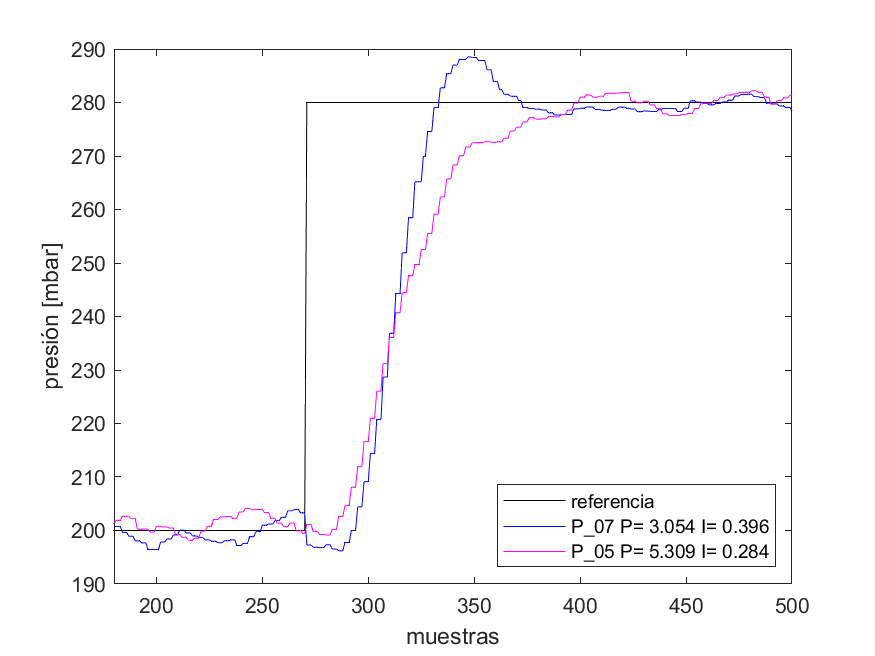
\includegraphics[width=80mm]{PIT1b.png}}
\hspace{-4mm}
	\subfigure[]{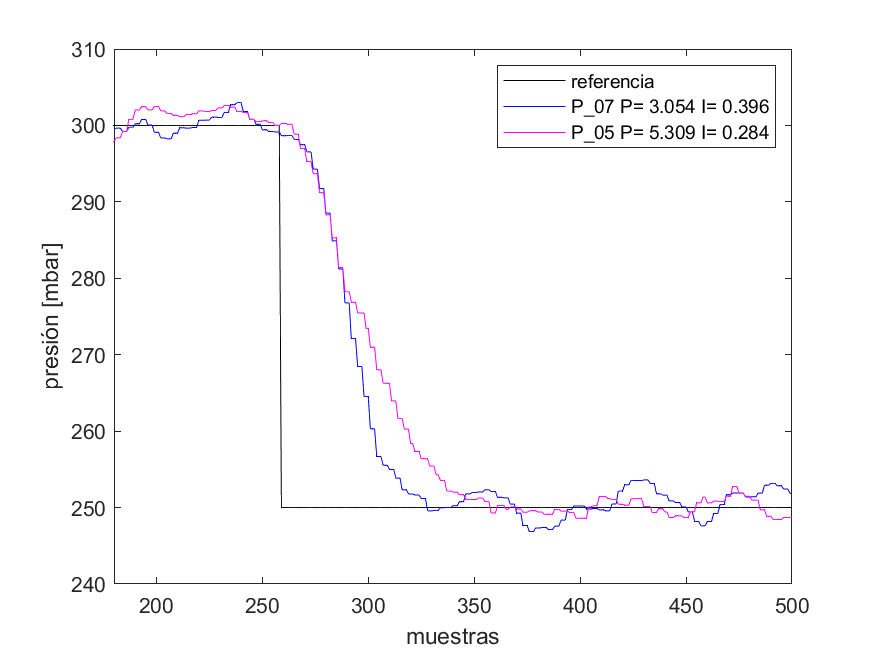
\includegraphics[width=80mm]{PIT1c.png}}
	\caption{Comparación PID para PIT01} \label{fig:PIT1}
\end{figure}

\begin{figure}[htbp]
	\centering
	\subfigure[]{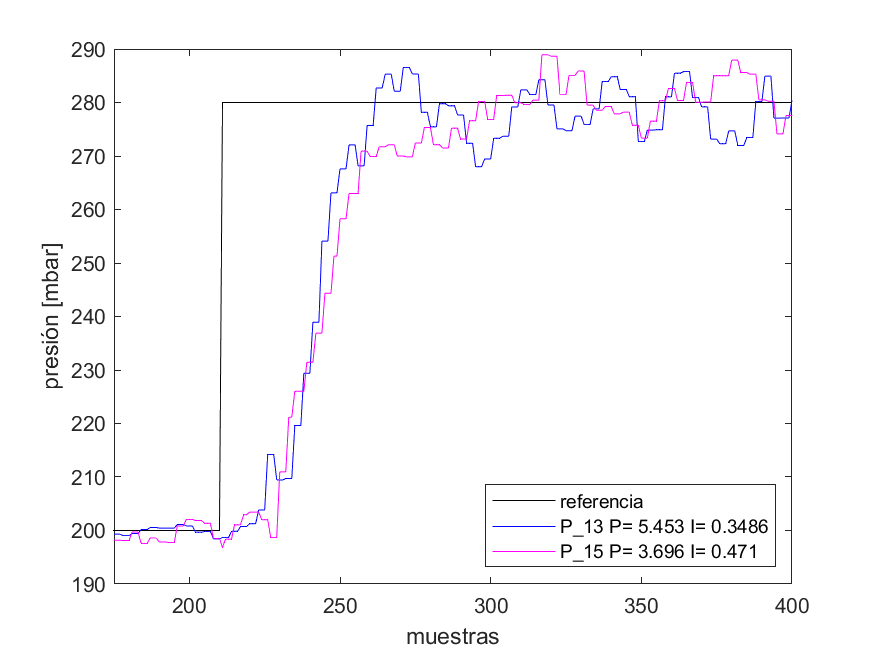
\includegraphics[width=80mm]{PIT2a.png}}
	\hspace{-4mm}
	\subfigure[]{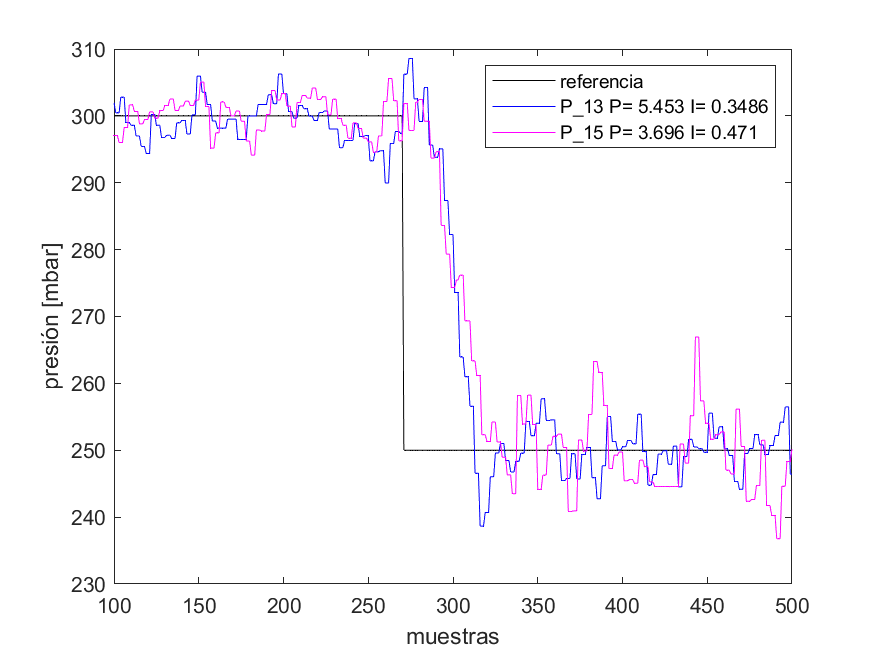
\includegraphics[width=80mm]{PIT2b.png}}
	\caption{Comparación PID para PIT02} \label{fig:PIT2}
\end{figure}


\subsubsection{Pruebas de control}
Para observar la respuesta del sistema de control se generaron perturbaciones con las válvulas del banco de prueba. FIGURA \ref{fig:pert1}
\begin{figure}[htb]
	\centering
	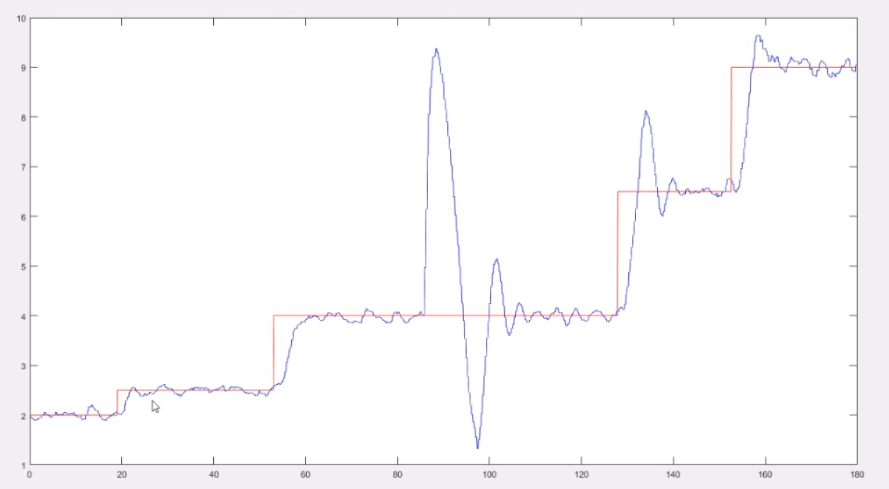
\includegraphics[width=0.9\linewidth]{pert1.png}
	\captionof{figure}{Comportamiento del sistema ante perturbaciones}
	\label{fig:pert1}
\end{figure}
\fcolorbox{red}{yellow}{poner con el diagrama de p Y id cual fue la q se cerró} acá solo se cerró


\subsubsection{Valores extremos/críticos de estudio}

\paragraph{Máxima presión}

Para esta prueba se llevó al motor a su máxima frecuencia (60Hz) de trabajo, se dejó la válvula FV03 totalmente abierta y se cerraron las válvulas FV01 y FV02 (Figura  \ref{fig:diag}). Esto provocó que la bomba llegue a su máxima presión que se obtiene al momento en que el caudal que circula por PIT01 se hace muy próximo a cero.\\
\textbf{\textit{Máxima presión:}} 938 mbar
\begin{figure}[h!]
	\centering
	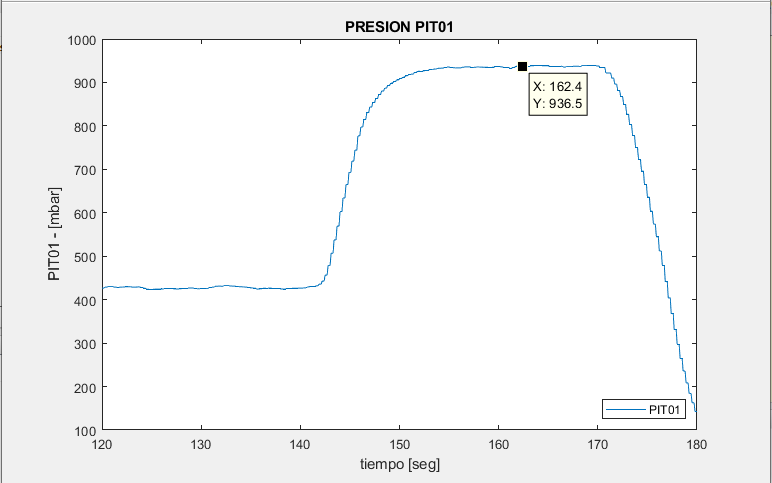
\includegraphics[width=0.9\linewidth]{Presion_Max.png}
	\captionof{figure}{Máxima presión}
	\label{fig:PMAX}
\end{figure}

\paragraph{Mínima presión}
Para obtener el valor de mínima presión de trabajo se configuró el VSD a 20 Hz y se abrieron todas las válvulas (Figura  \ref{fig:diag}), ésto generó que la bomba impulse el caudal con el menor esfuerzo. \\
\textbf{\textit{Mínima presión:}} 65,43 mbar
\begin{figure}[h!]
	\centering
	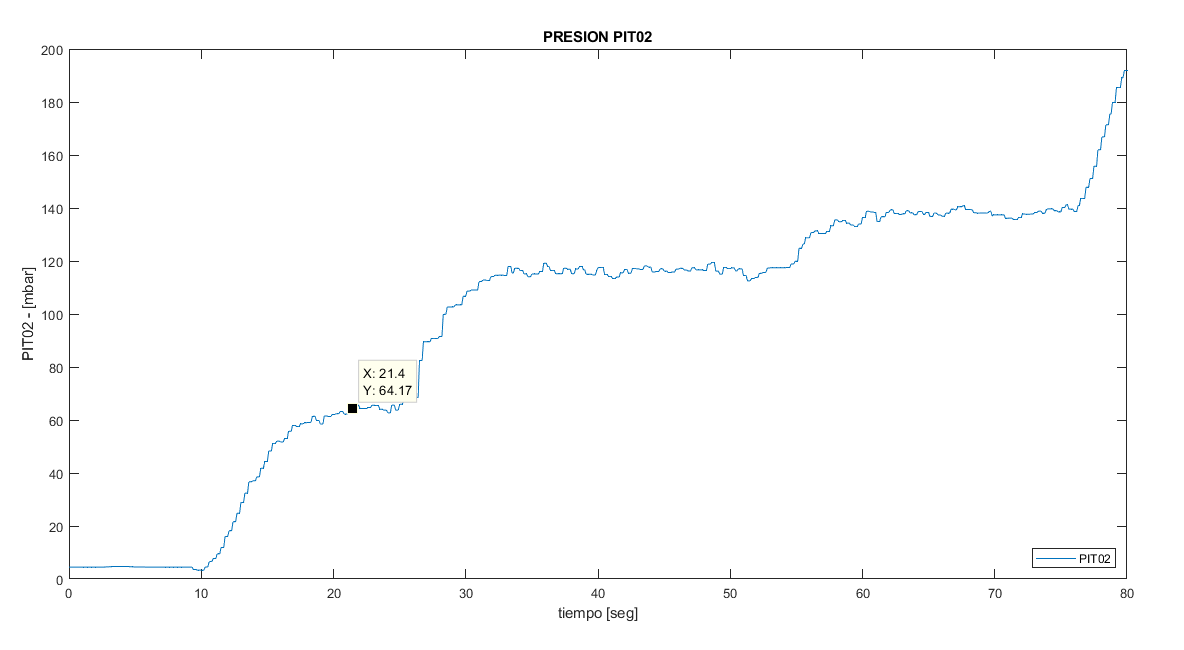
\includegraphics[width=0.9\linewidth]{Presion_Min.png}
	\captionof{figure}{Mínima presión}
	\label{fig:Pmin}
\end{figure}

\paragraph{Máximo caudal}
Para obtener el valor de caudal máximo se llevó al motor a su máxima frecuencia (60 Hz), se abrió completamente la válvula FV03 y FV02, y se cerró la válvula de BYPASS FV01 (Figura  \ref{fig:diag}).
Esto provoca que todo el caudal impulsado por la bomba circule por el caudalímetro FT01.\\
\textbf{\textit{Máximo caudal: }}11,69 L/min
\begin{figure}[h!]
	\centering
	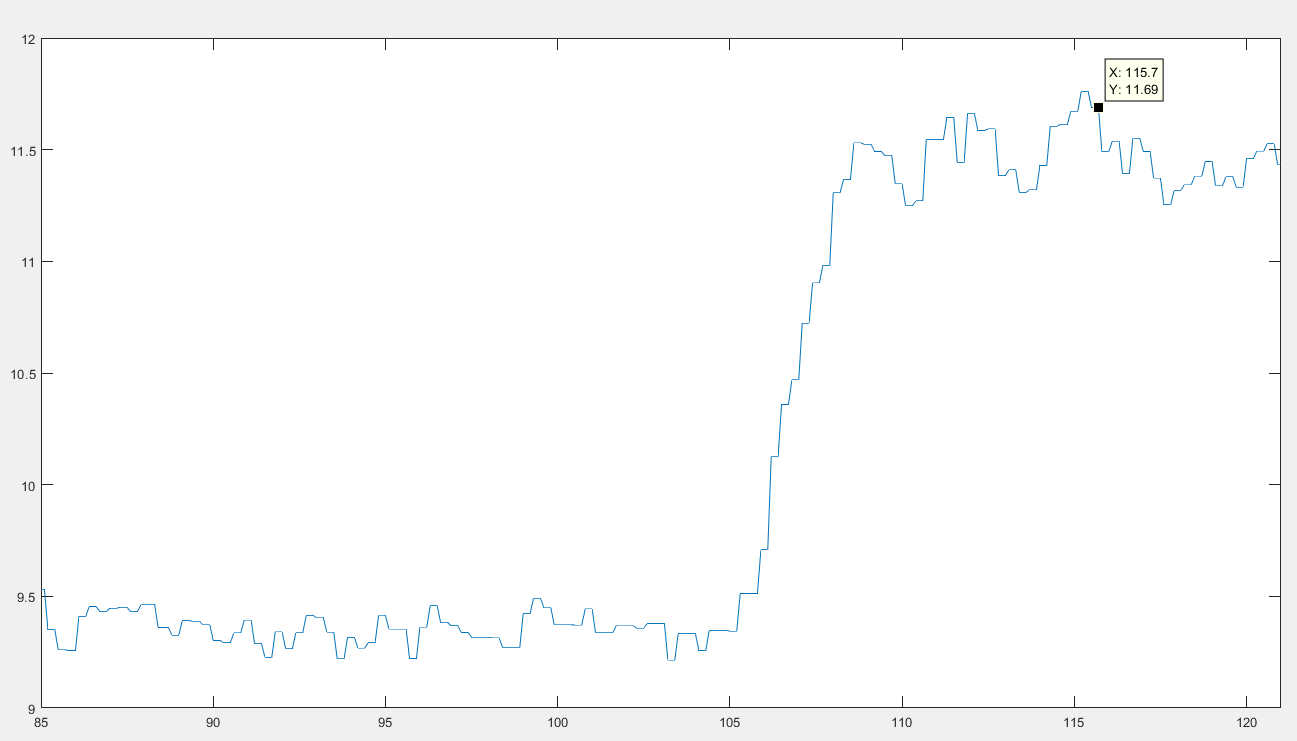
\includegraphics[width=0.9\linewidth]{Caudal_Max.png}
	\captionof{figure}{Máximo caudal}
	\label{fig:CM}
\end{figure}




\begin{comment}
\fcolorbox{red}{yellow}{Estuve viendo las curvas con escalones donde se ve que la ganancia estática se modifica frente a diferentes escalones. Si el objetivo fuese calcular un controlador para ese sistema una buena opción seria un controlador PI. De esta forma, la acción integral va a tratar de hacer que el error de estado estacionario sea cero frente a una entrada escalón. Además, los problemas que pueden existir en el envejecimiento de componentes, errores en el modelado y variaciones en la ganancia estática se van a mitigar con la parte integral del controlador. Obviamente al cambiar la planta la respuesta va a cambiar pero se va a cumplir la consigna de seguir la referencia. Para mostrar esto es posible calcular un controlador para un sistema y luego probar el controlador en los dos sistemas. Eso hice en el pdf que les adjunto con un sistema con 3 polos reales. Más detalles pueden encontrar en el libro de Ogata o Control avanzado de Karl Astrom, capitulo 3.
De esta forma, me da la sensación que para los objetivos de esta materia plantear un controlador PI para un controlador me parece bien.}
\end{comment}







\subsection{SCADA}
Para realizar la pantalla de supervisión, control y adquisición de datos operador se utilizó el software iFix perteneciente al grupo \textbf{General Electric}.

El sistema SCADA creado (Figura \ref{fig:scada1}) se dividió en las siguientes secciones:
\begin{itemize}
	\item Esquemático del circuito hidráulico físico con las variables de presión y caudal en tiempo real.
	\item Valores de funcionamiento del motor obtenidos por el variador de velocidad.
	\item Alarmero, dónde se observa de forma visual valores críticos alcanzados en el sistema.
	\item Indicador de modo de funcionamiento físico o remoto.
	\item Modo de control a lazo abierto o lazo cerrado.
	\subitem Para el modo de lazo cerrado se creó una ventana individual para cada sistema de presión y caudal.
	\item Pantalla para observar gráficos en tiempo real dónde se divide según la variable a observar, con botones para abrir el control PID del sistema.
	\item Pantalla donde se observa datos históricos y se puede generar un archivo \textit{.txt} con la información de la variable elegida en un determinado período de tiempo.
\end{itemize} 

\begin{figure}[htb]
	\centering
	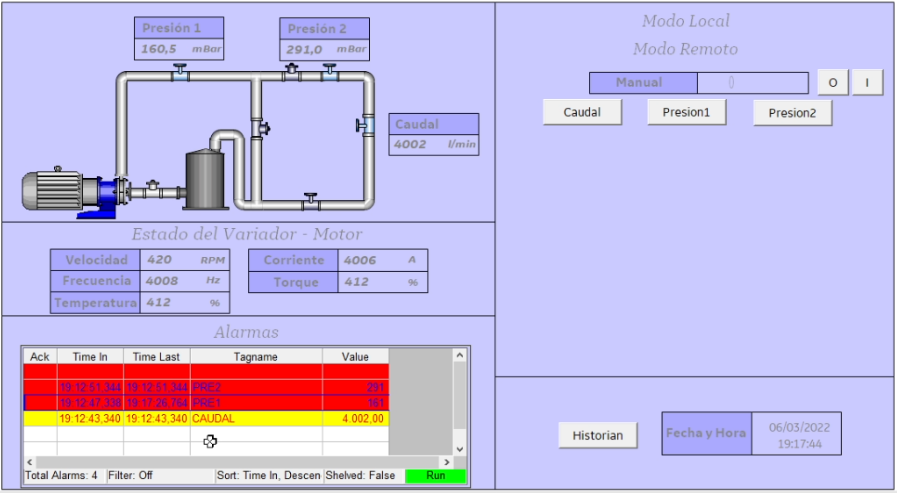
\includegraphics[width=0.9\linewidth]{scada1.png}
	\captionof{figure}{Pantalla SCADA}
	\label{fig:scada1}
\end{figure}


\subsubsection{Configuración driver Modbus}
Para realizar la configuración de cada ícono de la pantalla SCADA con su respectiva variable, se debió crear un MBE Driver (Figura \ref{fig:mbe}) dónde se estipula la dirección IP y el mapa de memoria con sus respectivas secciones que luego serán utilizadas por el DataBase (Figura \ref{fig:database}). 

Una vez creado el MBE Driver se debe generar la tabla \textit{DataBase} en dónde estará el nombre, dirección IP, tipo de elemento, descripción, alarma asociada, entre otros puntos de cada elemento.

La lista se encontrará unificada con las direcciones de \textit{UnityPro} (Tabla..\fcolorbox{red}{yellow}{..}).

\begin{figure}[h]
	\centering
	\includegraphics[width=0.9\linewidth]{mbe.png}
	\captionof{figure}{Configuración MBE}
	\label{fig:mbe}
\end{figure}
\begin{figure}[h]
	\centering
	\includegraphics[width=0.9\linewidth]{database.png}
	\captionof{figure}{Configuración MBE}
	\label{fig:database}
\end{figure}


\paragraph{Pruebas mediante ModSim}
Para realizar pruebas intermedias antes de unir SCADA con el programa del PLC se utilizó el software ModSim, dónde se generó los distintos mapas de memoria utilizados para modificar variables y observar el correcto funcionamiento de distintos elementos en el SCADA.

\begin{figure}[htb]
	\centering
	\includegraphics[width=0.9\linewidth]{modsim1.png}
	\captionof{figure}{ModSim}
	\label{fig:modsim1}
\end{figure}



\subsubsection{Alarmas y enclaves}
Dentro de la pantalla principal es posible observar el alarmero. El la tabla 
\fcolorbox{red}{yellow}{poner nombre tabla} se observa el diagrama causa efecto.

%Please add the following packages if necessary:
%\usepackage{booktabs, multirow} % for borders and merged ranges
%\usepackage{soul}% for underlines
%\usepackage[table]{xcolor} % for cell colors
%\usepackage{changepage,threeparttable} % for wide tables
%If the table is too wide, replace \begin{table}[!htp]...\end{table} with
%\begin{adjustwidth}{-2.5 cm}{-2.5 cm}\centering\begin{threeparttable}[!htb]...\end{threeparttable}\end{adjustwidth}
\begin{table}[!htp]\centering
	\caption{Generated by Spread-LaTeX}\label{tab: }
	\scriptsize
	\begin{tabular}{|l|r|r|r|r|r|r|r|r|r|r|r|r|r|r|r|r|r|}\toprule
		\multirow{2}{*}{\textbf{TAG INSTRUMENTO}} &\multirow{2}{*}{\textbf{SERVICIO}} &\multirow{2}{*}{\textbf{UNIDADES}} &\multicolumn{2}{c}{\textbf{RANGO}} &\multicolumn{4}{c}{\textbf{ALARMAS}} &\multicolumn{5}{c}{\textbf{ENCLAVAMIENTO}} &\textbf{EFECTO} &\multirow{2}{*}{\textbf{PROPOSITO DE ALARMA}} &\multirow{2}{*}{\textbf{CONSECUENCIA DE LA NO ACCION}} \\  \hline
		& & &\textbf{MIN} &\textbf{MAX} &\textbf{HI-HI} &\textbf{HI} &\textbf{LO} &\textbf{LO-LO} &\textbf{DELAY} &\textbf{HI-HI} &\textbf{HI} &\textbf{LO} &\textbf{LO-LO} &\textbf{VSD} & & \\  \hline
		\textbf{TT001} &\multirow{2}{*}{Temperatura} &\multirow{2}{*}{°C} &\multirow{2}{*}{} &\multirow{2}{*}{} & & &50 & & & & & & & &Informar alta temperatura del motor & \\  \hline
		\textbf{TT001} & & & & &70 & & & & &70 & & & &P &Informar muy alta temperatura del motor &Daño al bobinado \\  \hline
		\textbf{PIT001} &\multirow{2}{*}{Pre1} &\multirow{2}{*}{mbar} &\multirow{2}{*}{-1000} &\multirow{2}{*}{4000} &700 & & & & &700 & & & &P &Informar alta presión en cañería &Daño a bomba \\  \hline
		\textbf{PIT001} & & & & & & & & & & & & &<-1 &P &Informar desconexión PIT001 & \\  \hline
		\textbf{PIT002} &Pre2 &mbar &-1000 &4000 & & & & & & & & &<-1 &P &Informar desconexión PIT002 & \\  \hline
		\textbf{FT001} &Caudal &l/min &0 &60 & & &<0.5 & &30s & & &<0.5 & &P &Informar bajo flujo &Daño a bomba \\  \hline
		\textbf{VSD\_SC001} &Velocidad &rpm &0 &3600 &<200 & & & & &<200 & & & &P &Informar baja velocidad &Daño a motor \\  \hline
		\bottomrule
	\end{tabular}
\end{table}


\subsubsection{iHistorian}
\begin{figure}[htb]
	\centering
	\includegraphics[width=0.9\linewidth]{scada3.png}
	\captionof{figure}{Pantalla SCADA}
	\label{fig:scada3}
\end{figure}



\clearpage
\newpage


\newpage

\section{Mejoras futuras}
En un futuro se espera que alumnos de la carrera realicen mejoras en el banco de pruebas, por ejemplo:
\begin{itemize}
	\item Mejorar la distancia entre los sensores y los accesorios del sistemas, como válvulas o codos para que el fluido no se torne turbulento.
	\item Implementar sistemas sonoros o visuales de las alarmas.
	\item Generar una página web para observar los datos en tiempo real y/o manejar de forma remota.
	\item Realizar otro anexo no hidráulico para colocar al motor- variador y generar un nuevo banco de pruebas.
	\item Generar nuevas formas de perturbación a los sistemas.
	\item Implementar un sistema para controlar presión o caudal por medio de válvulas proporcionales.
	\item Realizar perturbaciones controladas y repetibles con válvulas proporcionales.
	\item Reemplazar bomba por una en mejor estado.
	\item Realizar pruebas de caudal y presión a mayor frecuencia.
\end{itemize}

\newpage
\section{Conclusiones}
Se concluye que el banco de pruebas construido es una herramienta útil para alumnos de las carreras de ingeniería que sigan ramas orientadas al control automatizado, ya que se tiene la posibilidad de generar perturbaciones en el sistema y observar distintas respuestas.

Se generó un sistema SCADA dónde se puede observar diversas variables en tiempo real y realizar estudios de ellas a través de datos históricos. Además, en la pantalla, se puede observar distintos tipos de anomalías causadas por el variador y los instrumentos utilizados en el proyecto, para facilitar la detección de errores y poder solucionarlos adecuadamente.

Se logró tener control eficaz sobre tres variables distintas mediante la variación de la frecuencia del motor, dónde esta es la única acción de control en el banco de pruebas.

Finalmente, la realización del proyecto tuvo un gran aporte para consolidar los conocimientos obtenidos durante la cursada de la materia \textit{Automatización Industrial} y también para el crecimiento personal y profesional.



\newpage
\clearpage
\newpage
\section{Referencias y Versiones de programas utilizados}


\printbibliography

\section*{Versiones de programas utilizados}

\begin{itemize}
	\item \textbf{\textit{Unity Pro XL}} (V11.0) Schneider Electric Industries SAS (2015) 
	\item \textbf{\textit{SoMove}} (V2.8.4.0) Schneider Electric Industries SAS (2020)  
	\subitem \textbf{\textit{Altivar DTM Library ATV31/312}} (V2.0.2.0) 
	\item \textbf{\textit{iFix Workspace}} (V6.0) General Electric Company (2018) 
	\item \textbf{\textit{Matlab}} (V2018a) MathWorks (2017)
	\subitem \textbf{\textit{Simulink}}  (V2018a) MathWorks (2017)
	
	\item \textbf{\textit{Proficy Historian}} (V4.5) General Electric Company (2011) 
	\item \textbf{\textit{OPC Factory Server}} (V3.6) Schneider Electric Industries SAS (2015)
	
\end{itemize}
\newpage
\appendix
\clearpage
%\addappheadtotoc
\appendix
%\appendixpage




\section{Anexo 2: Manual SCADA}
\subsection{Características generales}
\subsection{Pantallas}
\subsubsection{Pantalla principal}
\paragraph{Alarmas}
\subsubsection{Pantallas de control}
\subsubsection{Pantallas gráficas}
\paragraph{Gráficos en tiempo real}
\paragraph{Gráficos históricos}



\newpage


\end{document}